\documentclass[mat1]{fmfdelo}
\usepackage{graphicx}
\usepackage{cleverref}
\usepackage{dsfont}
\usepackage{tikz-cd}
\usepackage{ mathrsfs }

\graphicspath{ {./slike/} }

\makeatletter
\DeclareRobustCommand{\sqcdot}{\mathbin{\mathpalette\morphic@sqcdot\relax}}
\newcommand{\morphic@sqcdot}[2]{%
\sbox\z@{$\m@th#1\centerdot$}%
\ht\z@=.33333\ht\z@
\vcenter{\box\z@}%
}
\makeatother

\makeatletter
\DeclareRobustCommand{\k}{
    \mathcal{K}
}

\makeatletter
\DeclareRobustCommand{\h}{
    \mathcal{H}
}
\makeatletter
\DeclareRobustCommand{\si}{
    \bar{\sigma}
}


\DeclareMathOperator*{\supp}{supp}



\DeclareMathOperator*{\htt}{ht}

\makeatletter
\DeclareRobustCommand{\pot}{
    $\h-$pot
}



\newcommand\mymathop[1]{\mathop{\operatorname{#1}}}

\naslov{Minimalni končni modeli prostorov}
\title{Minimal finite models of spaces}
\avtor{Filip Bezjak}
\mentor{dr. Petar Pavešić}
\letnica{2023}
\klasifikacija{55U10}
\kljucnebesede{Končni topološki prostori, šibka homotopska ekvivalenca, homotopska ekvivalenca, delno urejene množice, simplicialni kompleksi, grafi, sfere}
\keywords{Finite topological spaces, weak homotopy equivalence, homotopy equivalence, partialy orderred sets, simplicial complexes, graphs, spheres}

\povzetek{Rečemo, da je končni topološki prostor model prostora, če mu je šibko homotopsko ekvivalenten. Model je minimalen, če ima izmed vseh modelov najmanjšo kardinalnost. Končnim $T_0$ topološkim prostorom lahko priredimo simplicialne komplekse. Eden izmed glavnih izrekov v delu nam pa pove, da je geometrijska realizacija tega kompleksa šibko homotopsko ekvivalentna začetnemu prostoru. S tem dobimo orodje za iskanje končnih modelov prostorov. V tem delu bomo poiskali minimalne modele topoloških sfer in končnih grafov.}

%  Prevod slovenskega povzetka v angleščino.
\abstract{We say, that finite topological space is a model of a topological space, if they are weak homotopy equvalent. A model is minimall, if it has the smallest cardinality of all models of a space. Every finite $T_0$ space has its asociated simplicial complex. One of the main theorems of this graduate thesis states, that the geometric realisation of the asociated simplicial complex is weak homotopy equivalent to the initial space. This gives us a tool to find finite models of spaces. In this thesis, we will find minimal models of of topological spheres and finite graphs}


\begin{document}

\tableofcontents

\section{Uvod}
Tema sodi na področje algebraične topologije na končnih prostorih. Topologije na končnih prostorih so večkrat spregledane, saj je vsaka $T_1$ topologija
na končnem prostoru diskretna. Če pa lastnosti $T_1$ ne zahtevamo, postanejo veliko bolj zanimive. Vsaka končna $T_0$ 
topologija nam enolično določa neko delno ureditev in obratno. Torej so končni topološki prostori in delne ureditve močno povezani. Tej povezanosti rečemo korenspodenca Alexandrova, ki jo bomo podrobneje predstavili v razdelku \ref{sec:delne}. Preden se lotimo minimalnih modelov prostorov, moramo najprej 
defnirati homotopsko in šibko homotopsko ekvivalenco \ref{sec:1} ter simplicialne komplekse \ref{sec:simpleks}. V razdelku \ref{sec:minimal} je dokazan glavni izrek \ref{iz:ksibka} dela, ki pravi, da je končen topološki prostor šibko homotopsko ekvivalenten geometrijski realizaciji 
prirejenega simplicialnega kompleksa. Ker delno urejene množice predstavimo s Hassejevim diagramom, bomo tudi končne topološke prostore predstavljali na tak način. Ker pa je šibki homotopski tip enodimenzionalnega prostora odvisen le od fundamentalne 
grupe, bomo vpeljali poti oziroma zanke v Hassejeve diagrame \ref{sec:hasse}. Grupa ekvivalenčnih razredov teh zank pa je izomorfna fundamentalni grupi prostora, kateremu smo priredili delno ureditev. Temeljni vir diplomskega dela je knjiga 
\textit{Algebraic Topology of Finite Spaces and Aplications} \cite{Solr-0000594456}.


\section{Homotopska in šibka homotopska ekvivalenca}\label{sec:1}

Ena izmed glavnih nalog algebraične topologije je iskanje prostorov, ki so si 
na nek način podobni oziroma ekvivalentni. Prvi pojem podobnosti, ki ga spoznamo
je homeomorfizem. Dva prostora sta homeomorfna, če lahko enega zvezno spremenimo v drugega in pri tem prostora ne lepimo in ga ne trgamo, oziroma če med njima obstaja homeomorfizem. Ekvivalenco med dvema 
prostoroma pa lahko definiramo na načine, ki so veliko širši kot homeomorfizem.
Na primer torus $S^1\times B^2$ in sfera $S^1$ imata podobno obliko, vendar nista
 homeomorfna. Zato bomo definirali homotopsko in šibko homotopsko ekvivalenco, ki bosta povezali prostore s podobnimi oblikami.

Spomnimo se, \textit{homotopija} je taka družina preslikav $f_t(x):X \rightarrow Y$, da je prirejena preslikava $F(x,t):X \times I \rightarrow Y$, definirana kot $F(x,t)=f_t(x)$, zvezna. Rečemo, da sta preslikavi $f_0$ in $f_1$ homotopni in pišemo $f_0 \simeq f_1$


\begin{definicija}
    Preslikava  $f : X \rightarrow Y$ je \textit{homotopska ekvivalenca} prostorov $X$ in $Y$, če obstaja preslikava $g: Y\rightarrow X$, taka da
    je $f g \simeq 1_Y$ in $gf \simeq 1_X$. Preslikavo $g$ imenujemo \textit{homotopski inverz od f}. Če taka preslikava $f$ obstaja, rečemo, da sta prostora $X$ in
    $Y$  \textit{homotopsko ekvivalentna}, oziroma, da imata isti \textit{homotopski tip}.
\end{definicija}

\begin{definicija}
    Naj bo $A \subseteq X$. Preslikavo $r : X \rightarrow A$ za katero 
    velja $r|_A = 1_A$ imenujemo \textit{retrakcija}, podprostor
     $A$ pa retrakt prostora $X$. Podprostor $A \subseteq X$ je 
     \textit{deformacijski retrakt}, če obstaja homotopija $H : X \times
      I \rightarrow X$ med $1_X$ in preslikavo $ir$, kjer je $r : X 
      \rightarrow A$ retrakcija, $i:A\rightarrow X$ pa inkluzija. Homotopijo $H$ imenujemo \textit{deformacijska 
      retrakcija}. Če homotopija $H$ miruje na množici $A$ jo imenujemo 
      \textit{krepka deformacijska retrakcija}, prostor $A$ pa 
      \textit{krepki deformacijski} retrakt prostora X. Za prostor $X$ rečemo, da je \textit{kontraktibilen}, če obstaja deformacijska retrakcija na točko. Oziroma, če je identiteta homotopna kaki konstantni preslikavi.
\end{definicija}

Če je $A\subseteq X$ in je $A$ deformacijski retrakt od $X$, potem sta 
$X$ in $A$ homotopsko ekvivalentna prostora. Res, če je $i:A\rightarrow
 X$ inkluzija, $r:X\rightarrow A$ retrakcija, potem je $ri=1_A$
  in $ir\simeq1_X$. Eden izmed načinov, da preverimo, ali sta
   prostora $A$ in $B$ homotopsko ekvivalentna, je, da poiščemo prostor
    $X$, ki vsebuje $A$ in $B$, kot deformacijska retrakta. 

Homotopija $f_t: X\rightarrow X$, ki nam da krepko deformacijsko retrakcijo 
prostora $X$ na podprostor $A$, ima lastnost, da velja 
$f_t|_A=1_A$, za vse $t$. V splošnem, homotopija 
$f_t:X\rightarrow Y$, katere zožitev na podprostor $A\subseteq X$ je 
neodvisna od $t$ imenujemo \textit{homotopija relativno A}. Krepka 
deformacijskia retrakcija $X$ na $A$ je torej homotopija med retraktom
 $ir$ in identiteto $1_X$, relativno $A$, kjer je $r:X\rightarrow A$ retrakt in $i:A\rightarrow X$ inkluzija.


\begin{figure}[h!]
    \centering
    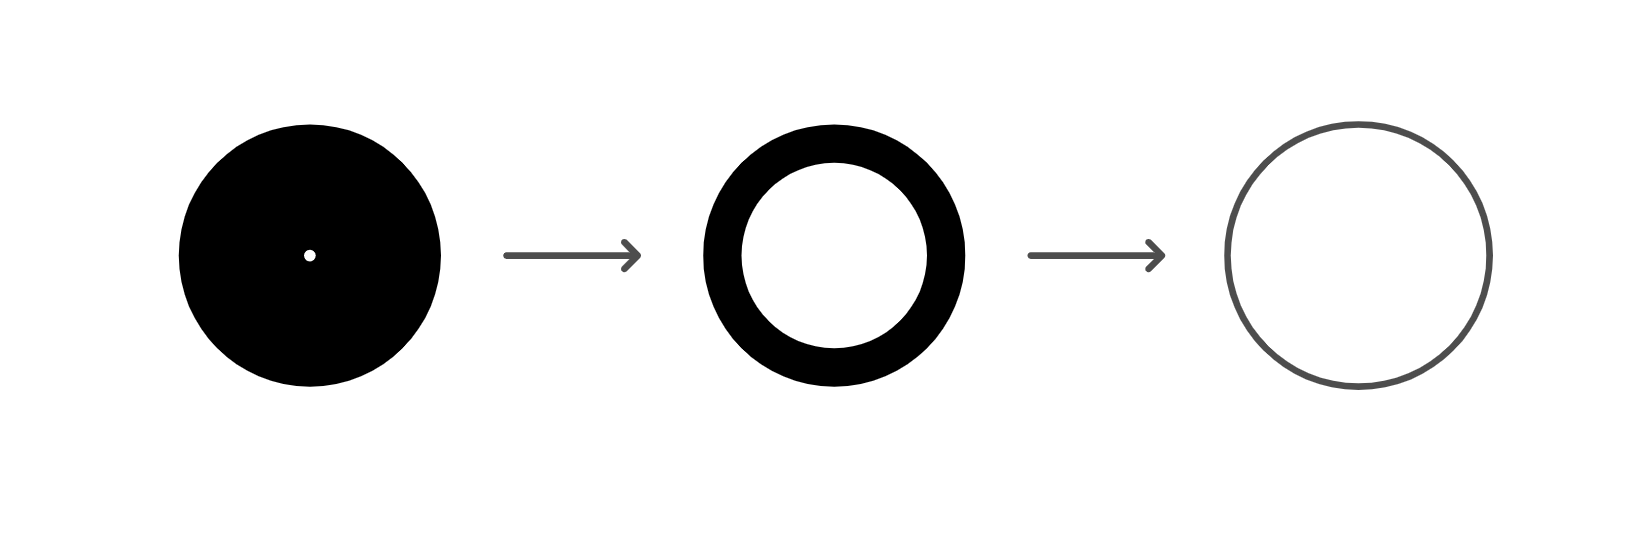
\includegraphics[width=1\linewidth]{def-retract.png}
    \caption{Punktiran disk se deformacijsko retrakira na robno sfero $S^1$}
\end{figure}

Šibko homotopsko ekvivalenco pa opišemo preko homotopskih grup, ki
 jih bomo definirali v nadaljevanju. Prva homotopska grupa se imenuje
  fundamentalna grupa. Je grupa ekvivalenčnih razredov zank v prostoru, 
 tj. poti z enako začetno in končno točko.

Pot v prostoru $X$ je zvezna preslikava $ f: I \rightarrow X$, pri čemer je $I$ enotski interval $[0,1]$. Poti sta homotopni, če lahko eno zvezno deformiramo v drugo, brez da bi premaknili krajišči poti.
\begin{definicija}
    
    Homotopija poti v $X$ je družina preslikav $f_t:I \rightarrow X, 0\le t \le 1$, taka da
    \begin{itemize}
        \item 
        sta krajišči $f_t(0) = x_0$ in $f_t(1) = x_1$ neodvisni od $t$ in
%t po homotopiji, s po intervalu poti
        \item 
        je prirejena preslikava $F:I\times X \rightarrow X$ definirana s $F(t,s) = f_t(s)$ zvezna.
    \end{itemize}
    Za poti $f_1$ in $f_0$, ki sta povezani s homotopiijo $f_t$ rečemo, da sta homotopni in označimo $f_1 \simeq f_0$.
\end{definicija}



\begin{trditev}
    Relacija homotopije na poteh s fiksnima krajiščema je ekvivalenčna relacija za vsak topološki prostor.
\end{trditev}

\begin{dokaz}
    Preveriti moramo 3 lastnosti ekvivalenčnih relacij, refleksivnost, simetričnost in tranzitivnost.

    Najprej preverimo refleksivnost. Naj bo $f : I \rightarrow X$ pot v prostoru $X$. Homotopijo definiramo kot $f_t(s)=f(s)$.
    
    Naj velja $f \simeq g$ in naj bo $f_t(s)$ homotopija med $f$ in $g$, 
    torej $f_0=f$ in $f_1=g$. Homotopijo med $g$ in $f$ definiramo kot 
    $g_t(s)=f_{1-t}(s)$. Velja $g_0=f_1=g$ in $g_1=f_0=f$. Ker je 
    $g_t(s)$ kompozitum zveznih preslikav, je zvezna. Sledi, da je 
    relacija homotopije simetrična.
    
    Naj bodo $f, g \text{ in } h$ poti v $X$ in naj velja $f \simeq g$ 
    in $g \simeq h$. Naj bo $f_t(s)$ homotopija med $f$ in $g$ in 
    $g_t(s)$ homotopija med $g$ in $h$. Definirajmo 
    $$h_t(s)=\begin{cases}
        f_{2t}(s), & t \in [0,\frac{1}{2}] \\
        g_{2t-1}(s), & t \in [\frac{1}{2},1]
    \end{cases}
    $$
    Velja $h_0=f_0=f$ in $h_1=g_1=h$. Ker je $h_t(s)$ sestavljena iz dveh zveznih poti, ki se ujemata na preseku, je zvezna, sledi, da je relacija tranzitivna.
\end{dokaz}

Za poljubni poti $f,g : I \rightarrow X$, za kateri velja $f(1) = g(0)$ 
lahko definiramo njun stik $f\sqcdot g$, ki preteče $f$ in $g$ z dvojno 
hitrostjo v enotskem intervalu.
$$ f\sqcdot g(s) \begin{cases}
    f(2s), &s \in [0,\frac{1}{2}] \\
    g(2s-1), & s \in [\frac{1}{2},1]
\end{cases}
$$

    Definirajmo še \textit{reparametrizacijo} poti $f$ kot kompozitum $f 
    \varphi$, kjer je $\varphi: I \rightarrow I$ neka zvezna preslikava, za 
    katero velja $\varphi(0)= 0$ in $\varphi(1)=1$. Reparametrizacija poti 
    ohranja homotopski razred, saj sta $f\varphi$ in $f$ povezani preko 
    $f\varphi_t$, pri čemer je $\varphi_t(s)=(1-t)\varphi(s)+ts$. Vidimo, da 
    $\varphi_t(s)$ leži med $\varphi(s)$ in $s$, torej na $I$, zato je 
    $f\varphi_t(s)$ dobro definirana.

Če se omejimo samo na poti $f:I \rightarrow X$ z enako začetno in končno točko $f(0) = f(1) = x_0$, govorimo o zankah, za $x_0$ pa rečemo, da je izhodišče.
Množico vseh homotopskih razredov $[f]$, z izhodiščem $x_0$ označimo s $\pi_1(X,x_0)$.

\begin{izrek}
    $\pi_1(X,x_0)$ opremljena s produktom $[f][g] = [f\sqcdot g]$ je grupa.
\end{izrek}

\begin{dokaz}
    Najprej preverimo dobro definiranost produkta. Naj velja $[f]=[f']$, preko homotopije $f_t$ in $[g]=[g']$ preko $g_t$. Potem sta $f\sqcdot g$ in $f'\sqcdot g'$ homotopni preko
    $h_t(s) =f_t \sqcdot g_t$. Vidimo, da $h_0=f_0 \sqcdot g_0=f \sqcdot g$ in $h_1=f_1 \sqcdot g_1=f'\sqcdot g'$. Ker je $f_t(1)=g_t(0)$ za vsak t in sta $f_t(s)$ in $g_t(s)$ zvezni, sledi, da je tudi $h_t(s)$ zvezna, torej velja [$f\sqcdot g$]=[$f'\sqcdot g'$].

    Naj bodo $f$, $g$ in $h$ poti v $X$ in naj bo $f(1)=g(0)$ in 
    $g(1)=h(0)$. Potem sta oba stika $(f\sqcdot g) \sqcdot h$ in 
    $f\sqcdot (g \sqcdot h)$ definirana, $(f\sqcdot g) \sqcdot h$ pa je
     reparametrizacija poti $f\sqcdot (g \sqcdot h)$ preko odsekoma linearne 
     funkcije
    $$
    \varphi(s)=\begin{cases}
        2s, & s \in [0,\frac{1}{4}]\\
        s+\frac{1}{4}, & s \in [\frac{1}{4},\frac{1}{2}]\\
        \frac{s}{2}+\frac{1}{2}, &s \in [\frac{1}{2},1] \\
    \end{cases}
    $$ zato sta poti homotopni, torej je množenje v $\pi_1(X,x_0)$ asociativno.

    Naj bo $f$ pot v $X$ in naj bo $c$ konstantna pot definirana s $c(s)=f(1)$, $fc$ je reparametrizacija $f$ preko 
    $$\varphi(s)=\begin{cases}
        2s, &s \in [0,\frac{1}{2}] \\
        1, & s \in [\frac{1}{2},1],\\
        \end{cases}
    $$zato velja $fc\simeq f$. Podobno velja tudi  $cf\simeq f$, kjer je $c$ konstantna pot $c(s)=f(0)$. Sklepamo, da je $c(s)=x_0$ dvostranska enota v grupi  $\pi_1(X,x_0)$

    Inverz poti $f$ definiramo kot $\bar{f}(s)=f(1-s)$. Definirajmo $h_t=f_t\sqcdot \bar{f_t}$, pri čemer je 
    $$
    f_t(s)=
    \begin{cases}
        f(s), &s \in [0,1-t] \\
        f(1-t), & s \in [1-t,1] \\
        \end{cases}
$$
Ker je $h_0=f\sqcdot \bar{f}$ in $h_1=f(0)=c$, sledi, da je $f\sqcdot \bar{f}$ homotopna konstantni poti v $x_0$. Če $f$ zamenjamo z $\bar{f}$, sledi, da $\bar{f}\sqcdot f\simeq c$, zato je $[\bar{f}]$ obojestranski inverz od $[f]$.
\end{dokaz}

Kot že povedano, tej grupi pravimo fundamentalna grupa prostora $X$, z izhodiščem $x_0$. $\pi_1(X,x_0)$ je prva v zaporedju analogogno definiranih homotopskih grup $\pi_n(X,x_0)$, pri katerih namesto iz $I$ slikamo iz $n$-dimenzionalne kocke $I^n$.


Naj bo $I^n$ $n$-dimenzionalna kocka. Rob $\partial I^n \text{ od } I^n$ je podprostor točk pri katerih je vsaj ena koordinata enaka $1$ ali $0$. Definirajmo $\pi_n(X,x_0)$, množico homotopskih razredov preslikav $f:(I^n,\partial I^n) \rightarrow (X,x_0)$ pri čemer velja $f(\partial I^n) = x_0$.


Za $n\ge 2$ posplošimo stik definiran pri fundamentalni grupi.
$$ f\sqcdot g(s) \begin{cases}
    f(2s_1,s_2,\ldots,s_n), & s_1\in [0,\frac{1}{2}] \\
    g(2s_1-1,s_2,\ldots,s_n), & s_1 \in [\frac{1}{2},1]
\end{cases}
$$

\begin{izrek}
    $\pi_n(X,x_0)$ opremljena s produktom $[f][g] = [f\sqcdot g]$ je grupa za vsak $n \in \mathds{N}$.
\end{izrek}

Dokaz te trditve je enak dokazu za $n=1$, saj je v stik poti vpletena le prva komponenta poti.

\begin{definicija}
    Topološka prostora $X$ in $Y$ sta \textit{šibko homotopsko ekvivalentna}, če obstaja preslikava $f:X\rightarrow Y$, ki inducira izomorfizen $\pi_1(X,x_0)\rightarrow \pi_1(Y,f(x_0))$ za vsak $n \in \mathbb{N}$. Preslikavi $f$ rečemo \textit{šibka homotopska ekvivalenca.}
\end{definicija}



Homeomorfni prostori so homotopsko ekvivalentni, homotopsko ekvivalentni prostori so tudi šibsko homotopsko ekvivalentni. Obratno v splošnem ne velja.

Šibke homotopske ekvivalence imajo lastnost \textit{$2$ od $3$}, kar pomeni, da če sta dve od treh preslikav $f$, $g$ in $fg$ šibki homotopski ekvivalenci, potem je tudi tretja.
\section{Simplicialni kompleksi}\label{sec:simpleks}

\textit{Simpleks} ali $n$-simpleks je $n$-razsežni analog trikotnika. Točka je $0$-simpleks, $1$-simpleks je daljica, $2$-simpleks je trikotnik,
$3$-simpleks je tetraeder. $n$-simpleks definiramo kot množico svojih $n+1$ oglišč. \textit{Simplicialni kompleks $K$} je sestavljen iz množice oglišč $V_K$ in množice simpleksov $S_K$, sestavljene iz končnih nepraznih podmnožic od $V_K$, pri čemer je vsak element $S_k$ simpleks in vsaka podmnožica simpleksa je simpleks. Pišemo $\sigma \in K$ in $v \in K$, če je $\sigma \in S_K$ ter $v \in V_K$. Dimenzija $K$ je enaka maksimumu dimenzij njegovih simpleksov, $n$-dimenzionalnemu simpleksialnemu kompleksu rečemo tudi \textit{n-kompleks}. Omejili se bomo samo na končne komplekse, torej $n \in \mathbb{N}$.

Če je simpleks $\sigma$ vsebovan  v simpleksu $\tau$, mu rečemo \textit{lice} od $\tau$, rečemo mu \textit{pravo lice}, če $\tau\neq \sigma$. 
Simpleksu rečemo \textit{maksimalen simpleks}, če ni pravo lice nobenemu drugemu simpleksu. Subkompleks $L\in K$ simplicialnega kompleksa
 $K$ je simplicialni kompleks, tak da $V_L\subseteq V_K$ in $S_L\subseteq S_K$


Naj bo $\sigma = \{v_0,v_1,\ldots,v_n\}$ $n$-simpleks. Zaprt
simpleks $\bar{\sigma}$ je množica formalnih konveksnih kombinacij $\mymathop{\Sigma}_{i=0}^{n}\alpha_i v_i$
pri čemer je $\alpha_i \ge 0$ za vsak $0\le i \le n$ in $\mymathop{\Sigma}_{i=0}^{n}\alpha_i = 1$. Zaprt simpleks je metričen prostor z metriko

\begin{equation}
    \label{eq:metrika}    
d(\mymathop{\Sigma}_{i=0}^{n}\alpha_i v_i,\mymathop{\Sigma}_{i=0}^{n}\beta_i v_i) = \sqrt{\mymathop{\Sigma}_{i=0}^{n}(\alpha_i - \beta_i)^2}.
\end{equation}
Če so $v_i$ linearno neodvisne točke v $\mathbb{R}^m$ za nek $m\geq n$, potem je $\bar{\sigma}$ homeomorfen prostoru 
$\{\mymathop{\Sigma}_{i=0}^{n}\alpha_i v_i, | \mymathop{\Sigma}_{i=0}^{n}\alpha_i = 1 \text{ in } \alpha_i \ge 0 \}\subseteq \mathbb{R}^m$, 
kar pomeni, da lahko vsak zaprt simpleks predstavimo kot podprostor $\mathbb{R}^m$ z evklidsko topologijo.

\textit{Geometrijska realizacija} $|K|$ simplicialnega kompleksa $K$ je 
množica formalnih konveksnih kombinacij $\underset{v \in K}{\Sigma}\alpha_v v$, takih da je $\{v | \alpha_v > 0\}$ simpleks v $K$ in 
$\mymathop{\Sigma}_{v\in K}\alpha_v=1$. Rečemo, da $|K|$ realizira $K$. Za točko $x\in |K|$ označimo $\supp(x)=\{v | \alpha_v > 0\}$, 
tej množici pravimo nosilec od $x$. Topologijo na $\si$ definiramo na naslednji način. $U \subseteq |K|$ je odprta, natanko tedaj, ko je $U \cap 
\si$ odprta, za vsak $\sigma \in K$. Kot prej, če so $v\in K$ linearno neodvisne točke v $\mathbb{R}^m$ za nek $m\geq |V_K|$, potem je 
$|K|$ homeomorfen prostoru $\{\mymathop{\Sigma}_{v\in K}\alpha_v v | \mymathop{\Sigma}_{v\in K} \alpha_v = 1 \text{, } \alpha_i
\ge 0 \text{ in } \{v | \alpha_v > 0\} \text{ je simpleks v $K$}\} \subseteq \mathbb{R}^m$, kar spet pomeni, da lahko vsak simplicialni
kompleks predstavimo kot podprostor v $\mathbb{R}^{|V_K|}$ z evklidsko topologijo.
Če $L\subseteq K$, potem je $|L|\subseteq |K|$ zaprta podmnožica.

\begin{opomba}
    Če je $K$ $n-$kompleks, potem se ga da realizirati v $\mathbb{R}^{2n+1}$. To pomeni, da obstaja podprostor v
    $\mathbb{R}^{2n+1}$, ki je homeomorfen $|K|$. Vsak graf je geometrijska realizacija $1-$kompleksa, zato ga 
    lahko realiziramo v $\mathbb{R}^{2\cdot 1 +1}=\mathbb{R}^{3}$, kar je pa znano dejstvo iz teorije grafov.
\end{opomba}


\textit{Polieder} je geometrijska realizacija Simplicialnega kompleksa $|K|$, \textit{triangulacija} poliedra $X$ pa je simplicialni kompleks, katerega geometrijska realizacija je homeomorfna $X$.

Ker topologija na $|K|$ sovpada z topologijo na $\bar{\sigma}$, za vsak $\sigma\in K$ in je $U \subseteq |K|$ odprta, natanko tedaj, ko je $U \cap 
\si$ odprta, za vsak $\sigma \in K$, sledi, da je preslikava $f$ iz $|K|$ v nek topološki prostor $X$ zvezna, natanko tedaj, ko je $f|_{\bar{\sigma}}: \bar{\sigma} \rightarrow X$ zvezna za vsak $\sigma\in K$. Tudi $H:|K|\times I \rightarrow X$ je zvezna, natanko tedaj, ko je zvezna $H|_{\si\times I}:\si\times I \rightarrow X$, za vsak $\sigma\in K$.


\textit{Simplicialna preslikava} $\varphi :K \rightarrow L$, med 
simplicialnima kompleksoma $K$ in $L$, je preslikava med 
oglišči, $V_K \rightarrow V_L$, ki slika simplekse v 
simplekse. Preslikava $\varphi$ inducira zvezno preslikavo med 
kompleksoma $|\varphi| :|K| \rightarrow |L|$, kot $|\varphi|:
\underset{v \in K}{\Sigma}\alpha_v v \mapsto
\underset{v \in K}{\Sigma}\alpha_v \varphi(v)$.

    
\textit{Baricentrična subdivizija} simplicialnega kompleksa 
$K$ je simplicialni kompleks $K'$, čigar oglišča so 
simpleksi $\sigma \in K$, simpleksi v $K'$ so pa verige 
simpleksov v $K$, urejenih z inkluzijo. Torej $\sigma' \in K'$, če $\sigma' = \{\sigma_0, \sigma_1,...,\sigma_n\}$ in $\sigma_0\subsetneq \sigma_1\subsetneq...\subsetneq\sigma_n$. \textit{Težišče} simpleksa $\sigma \in K$ je točka $b(\sigma)=\underset{v\in \sigma}{\Sigma} \frac{v}{\#\sigma}$.

Definirajmo linearno preslikavo $S_K: |K'| \rightarrow |K|$, s predpisom $S_K(\sigma) = b(\sigma)$. Linearnost pomeni, da velja $S_K(\underset{\sigma\in \sigma'}{\Sigma} a_\sigma \sigma) =  \underset{\sigma\in \sigma'}{\Sigma} a_\sigma S_K(\sigma).$

\begin{primer}
Naj bo $K=\sigma=\{\{a\},\{b\},\{c\},\{a,b\},\{a,c\},\{b,c\},\{a,b,c\}\}$ 

$3-$simpleks.
\begin{figure}[h]
    \centering
    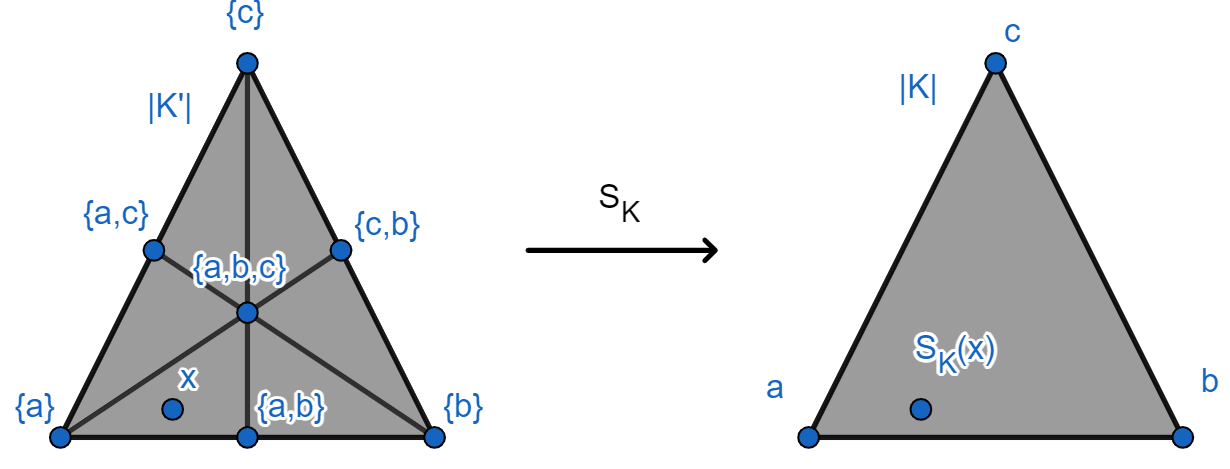
\includegraphics[width=0.7\linewidth]{sk.png}
\end{figure}
Poglejmo si preslikavo $S_K: |K'| \rightarrow |K|$. Naj bo $x$ tako kot na sliki. %Zaradi preglednosti označimo

Potem je 
$K'_x:=\supp(x)=\{\{a\},\{a,b\},\{a,b,c\}\}$ in $x= \underset{\sigma\in K'_x}{\Sigma} \alpha_{i_\sigma} \sigma$. Zato

\begin{align*}
S_K(x)&=S_K(\underset{\sigma\in K'_x}{\Sigma} \alpha_{i_{\sigma}} 
 \sigma) =  \underset{\sigma\in K'_x}{\Sigma} \alpha_{i_{\sigma}} 
S_K(\sigma)\\
&=\alpha_1S_K(\{a\})+\alpha_2S_K(\{a,b\})+\alpha_3S_K(\{a,b,c\}) \\ 
&=\alpha_1a+\alpha_2\frac{a+b}{2}+\alpha_3\frac{a+b+c}{3}.
\end{align*}
Preslikava $S_K$ je očitno homeomorfizem.



\end{primer}


\begin{trditev}\label{tr:shom}
    Naj bosta $K$ in $L$ simplicialna kompleksa in naj bosta $f,g:|K|\rightarrow |L|$ taki zvezni preslikavi, da za vsak $x\in |K|$ obstaja $\sigma \in L$, da $f(x),g(x) \in \overline{\sigma}.$ Potem sta $f$ in $g$ homotopni.
\end{trditev}

\begin{dokaz}
    Preslikava $H:|K|\times I\rightarrow |L|$, definirana kot $H(x,t)=tg(x) + (1-t)f(x)$ je dobro definirana, ker $f(x)$ in $g(x)$ ležita v istem zaprtem simpleksu. $H$ je zvezna, natanko tedaj, ko je zvezna $H|_{\overline{\sigma}\times I}:\overline{\sigma}\times I \rightarrow |L|$, za vsak $\sigma \in K$. Ocenimo 
\begin{align*}
    d(H(x,t)&,H(y,s)\leq d(tg(x)+(1-t)f(x),sg(x)+(1-s)f(x)) \\
&+d(sg(x)+(1-s)f(x),sg(y)+(1-s)f(y))\\
&\leq 2|t-s|+d(f(x),f(y))+d(g(x),g(y)).
\end{align*}
Torej zveznost $H$ sledi iz zveznosti $f$ in $g$.
\end{dokaz}

\begin{definicija}
    Simplicialni preslikavi $\varphi, \psi:K\rightarrow L$ sta \textit{kontiguentni}, če je za vsak $\sigma \in K$, $\varphi(\sigma)\cup \psi(\sigma)$ simplek sv L.
\end{definicija}

Če sta $\varphi$ in $\psi$ kontiguentni, potem $|\varphi|$ in $|\psi|$ zadostita predpodstavkam v trditvi \ref{tr:shom}, saj če $x\in \overline{\sigma}$, potem $|\varphi|(x)$ in $|\psi|(x)$ ležita v $\overline{\varphi(\sigma)\cup\psi(\sigma)}$. Takoj sledi naslednja posledica.

\begin{posledica}
    Če sta $\varphi$ in $\psi$ kontiguentni, sta $|\varphi|$ in $|\psi|$ homotopni.
\end{posledica}

\textit{Simplicialni stožec z vrhom $v$} je simplicialni kompleks $K$ z ogliščem $v$, za katerega velja, da je $\sigma \cup \{v\}$, za vsak simpleks $\sigma\in K$.

\begin{posledica}
    \label{pos:kontr}
    Če je $K$ simplicialni stožec, potem je $|K|$ kontraktibilen.
\end{posledica}

\begin{dokaz}
    Naj bo $v$ vrh od $|K|$. Po definiciji simplicialnega stožca, je simplicialna preslikava, ki slika vsako oglišče v $v$, kontiguentna identiteti. Zato je identiteta v $|K|$ homotopna konstantni preslikavi.
\end{dokaz}


\subsection{Poti v simplicialnem kompleksu}

\textit{Rob} simplicialnega kompleksa $K$ je urejeni par $e=(v_0,v_1)$, tak da je $\{v_0,v_1\}$ Simpleks v $K$. Oglišču $v_0$ rečemo \textit{začetek} $e$ in označimo 
$v_0=\mathfrak{o}(e)$, oglišču $v_1$ pa \textit{konec} od $e$, 
označimo $\mathfrak{e}(e)=v_1$. \textit{Lomljenka} dolžine $n$ je zaporedje
$(e_0,e_1,...,e_{n})$ robov v $K$ (lahko tudi prazno), za katerega velja, da je $\mathfrak{e}(e_i)=\mathfrak{o}(e_i+1)$, za vsak $0\leq i \leq n-1$
Lomljenka je sklenjena, če $\mathfrak{e}(e_0)=\mathfrak{o}(e_n)v_0$, Oglišču $v_0$ rečemo izhodišče. Če sta $\xi =(e_0,e_1,...,e_n)$ in $\xi'=(e'_0,e'_1,...,e'_{m})$, in velja $\mathfrak{e}(e_n)=\mathfrak{o}(e'_0)$ definiramo stik lomljenk $\xi\xi'$ kot $(e_0,e_1,...,e_{n}e'_0,e'_1,...,e'_{m})$.

Lomljenki $\cdots(v_i,v_{i+1})(v_{i+1},v_{i+2})\cdots$ in $\cdots(v_i,v_{i+2})\cdots$ sta preprosto ekvivalentni,če je $\{v_i,v_{i+1},v_{i+2}\}$ simpleks v $K$. Lomljenki $\xi_0$ in $\xi_n$ sta ekvivalentni, če obstaja zaporedje lomljenk $\xi_0\xi_1\cdots\xi_n$, pri katerem sta $\xi_i$ in $\xi_{i+1}$ preprosto ekvivalentni za vsak $0\leq i < n$


\begin{figure}[h]
    \centering
    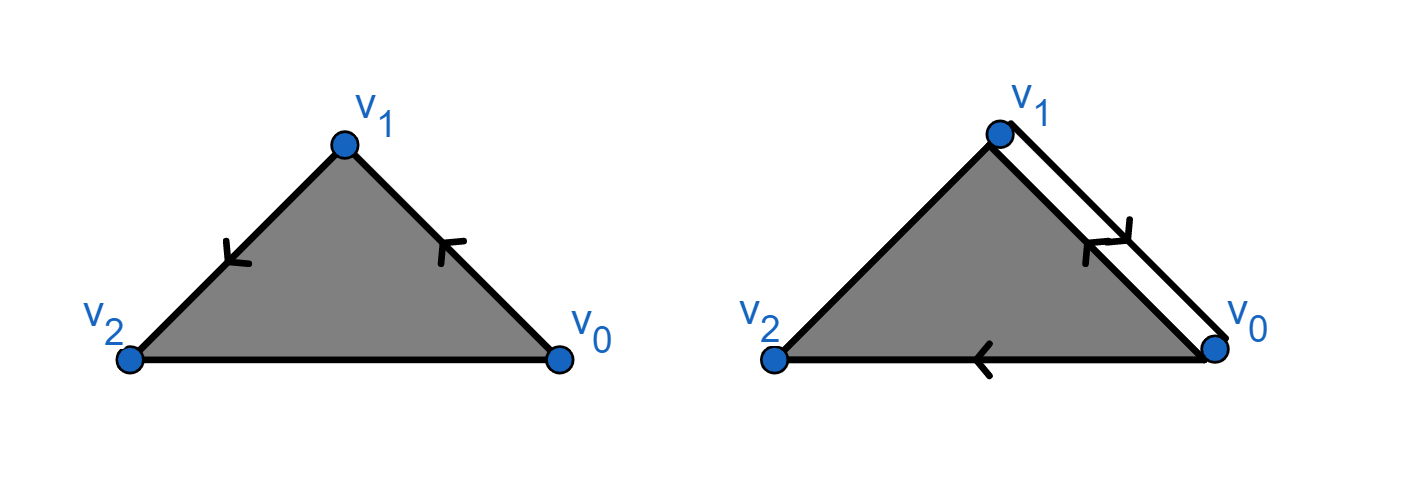
\includegraphics[width=0.9\linewidth]{lomljenki2.png}
    \caption{lomljenki $(v_0,v_1)(v_1,v_2)$ in $(v_0,v_1)(v_1,v_0)(v_0,v_2)$ sta ekvivalentni.}
\end{figure}

    Naj bo $K$ simplicialni kompleks in $v_0$ oglišče v $K$. Z $E(K,v_0)$ označimo množico ekvivalenčnih razredov sklenjenih lomljenk z izhodiščem v $v_0$. Ekvivalenčni razred sklenjene lomljenke $\xi$ označimo z $[\xi]$. Ekvivalenčni razred prazne lomljenke $[\emptyset]$ je $[(v_0,v_0)]$.

    \begin{trditev}
        Množica $E(K,v_0)$ z množenjem, ki ga inducira stik lomljenk, tvori grupo.
    \end{trditev}
\begin{proof}
    Dobra definiranost množenja in asociativnost sta očitni. 
    Identiteta je ekvivalenčni razred poti $(v_0,v_0)$. Inverz 
    od $(e_0,e_1,...,e_{n-1},e_n)$ je $(e^{-1},e^{-1}_{n-1},...,e^{-1}_1,$ $e^{-1})$, kjer $(v_i,v_{i+1})^{-1}=(v_{i+1},v_i)$.
\end{proof}

\begin{izrek}
    \label{iz:grupa lomljenk}
$E(K,v_0)$ je izomorfna $\pi_1(|K|,v_0)$
\end{izrek}

Dokaz lahko najdemo v \cite{spanier1995algebraic}
\section{Končni topološki prostori in delno urejene množice}
\label{sec:delne}

\textit{Končni topološki prostor} je topološki prostor s končno mnogo točkami, 
\textit{šibko urejena} množica je množica s tranzitivno in z refleksivno relacijo. Če je relacija še antisimetrična, dobimo \textit{delno} ureditev.
\\ \indent Naj bo $X$ končni topološki prostor. Za vsako točko $x \in X$ obstaja najmanjša odprta množica $U_x$, ki jo
vsebuje, oziroma presek vseh odprtih množic, ki vsebujejo $x$. Ta množica je odprta, saj je topologija zaprta za končne preseke.
    Točke uredimo s pravilom $ x\le y \text{, če } U_x \subseteq  U_y$. S tem dobimo šibko ureditev. 
    Antisimetričnost po definiciji sovpada z lastnostjo $T_0$, zato, relacija postane delna ureditev,
     natanko takrat, ko je topologija $T_0$.
    \\ \indent Obratno, naj bo $X$ šibko urejena množica. Na njej lahko definiramo topologijo z bazo $\{y \in X | y\le x\}_{x \in X}$. Če je
$y \le x$, je $y$ vsebovan v vsaki bazni množici, ki vsebuje $x$, torej je $y \in U_x$. Po drugi strani, če je $y\in
U_x$, potem je $y \in \{y \in X | y \le x\}$, torej velja, da je $y \le x$ natanko tedaj, ko je $y \in U_x$. Iz tega je razvidno, da so končni prostori in šibke ureditve enaki objekti, gledani z drugačnega stališča.


Delno urejene množice praviloma predstavljamo s Hassejevimi diagrami.

\begin{definicija}
    \textit{Hassejev diagram} delno urejene množice $X$ je usmerjen graf, katerega oglišča so točke, povezave pa so urejeni pari $(x,y)$, taki, da je  $x<y$ in ne obstaja tak $z$, da bi veljalo $x<z<y$.
\end{definicija}

Povezave $(x,y)$ ne rišemo s puščico iz $x$ v $y$, ampak bomo $x$ in $y$ povezali z ravno črto in $y$ pisali nad $x$. Če je $(x,y)$ povezava v Hassejevem diagramu končne delno urejene množice, rečemo, da $y$ \textit{pokrije} $x$ in pišemo $x\prec y$.

\begin{primer}
    Naj bo $X=\{a,b,c,d\}$ končen prostor, s topologijo 
    $\tau=\{\emptyset,X,\{b,d\},$ $\{c\},\{d\},\{b,c,d\},
    \{c,d\}\}$. Topologija je $T_0$, zato je $X$ tudi delno 
    urejena množica.
\begin{figure}[h!]
    \centering
    \begin{minipage}{0.5\textwidth}
        \centering
        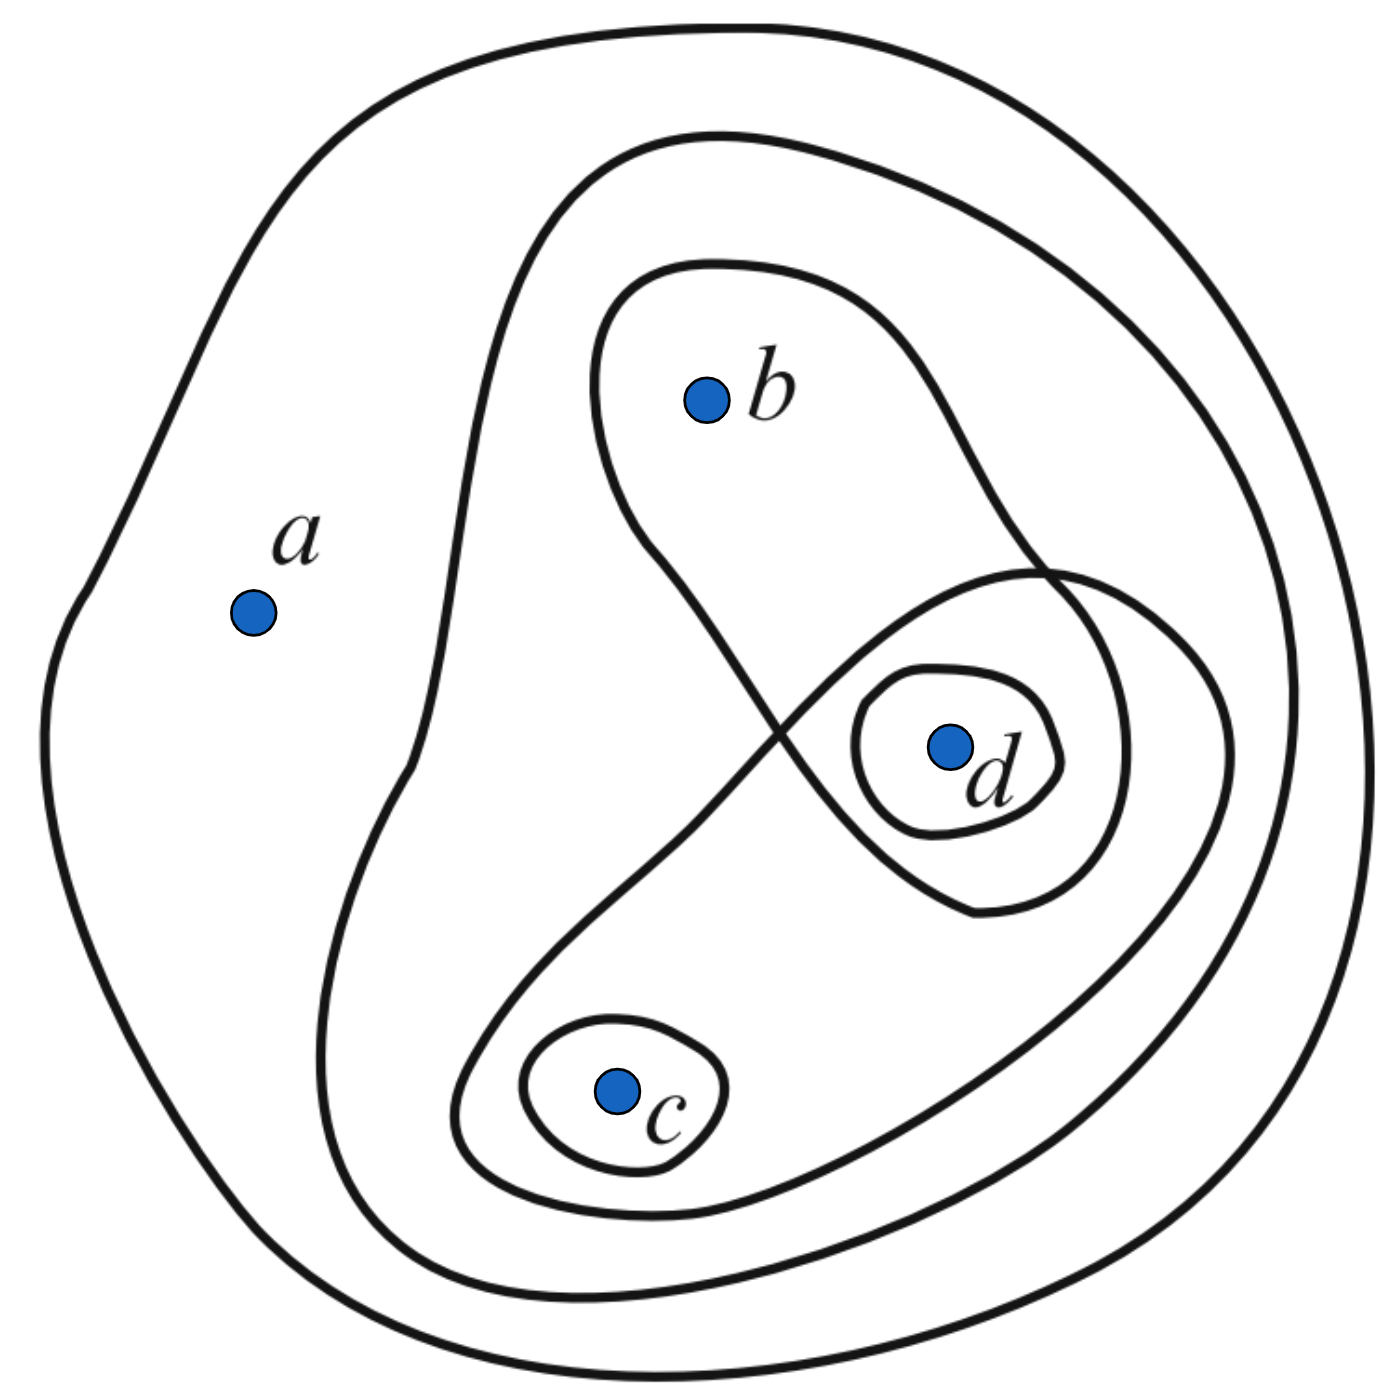
\includegraphics[width=0.6\linewidth]{open.png}
    \end{minipage}%
    \begin{minipage}{0.5\textwidth}
        \centering
        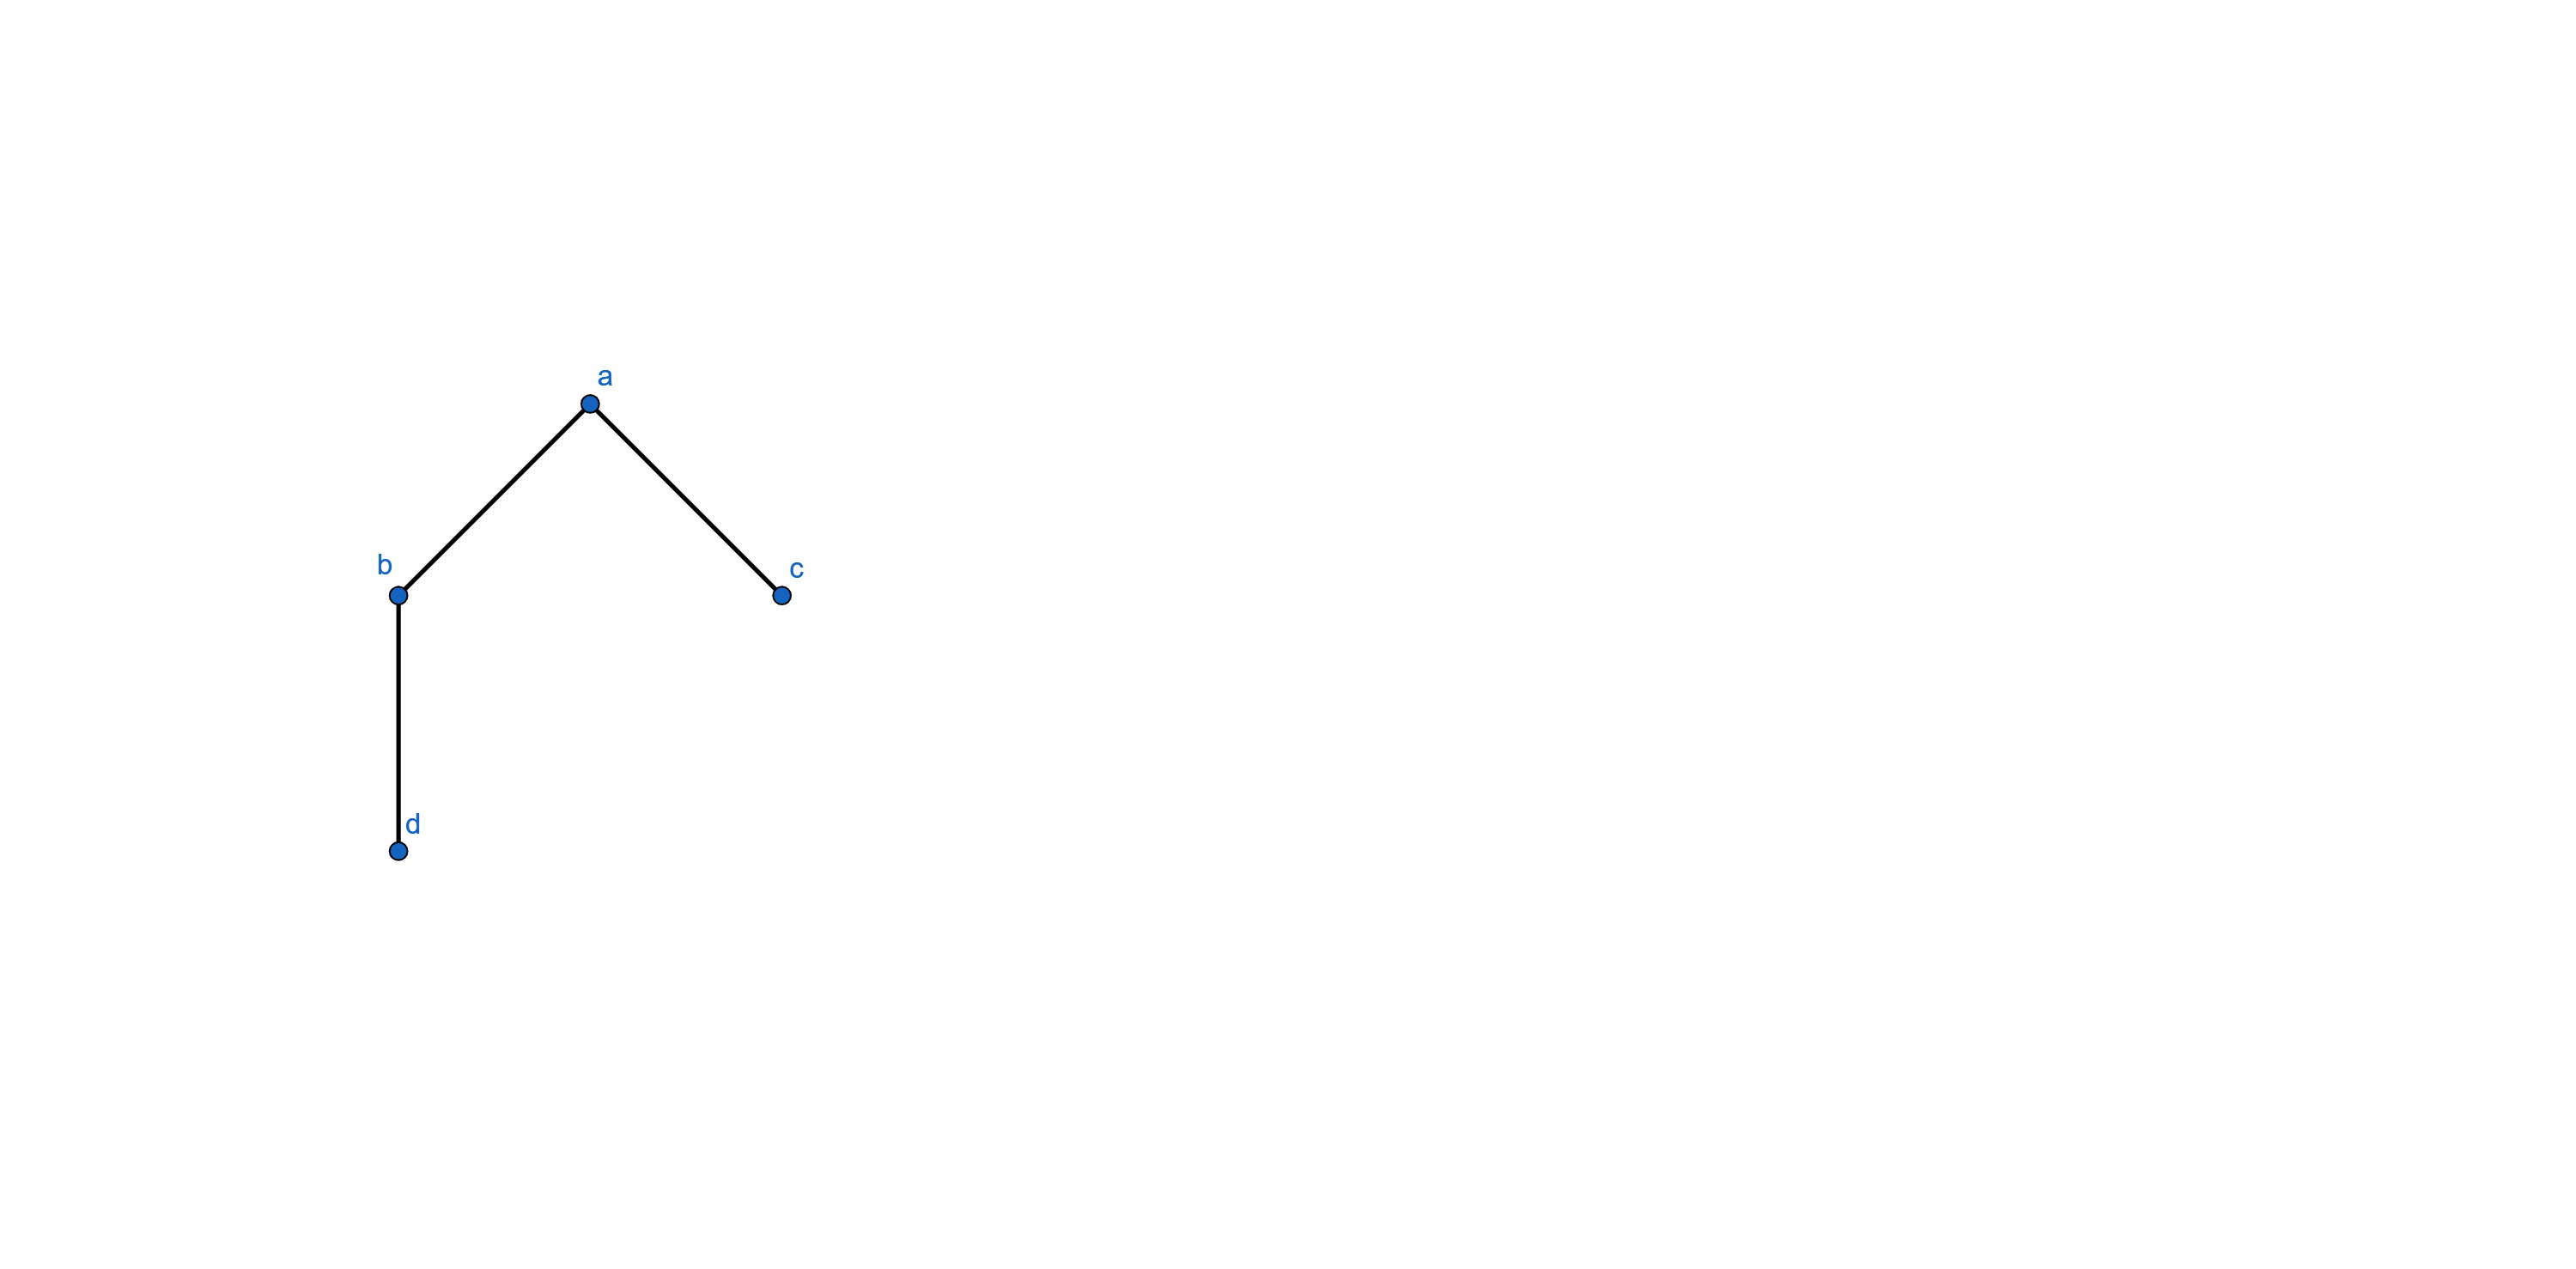
\includegraphics[width=2.5\linewidth]{hasse.png}
    \end{minipage}
    \caption{Odprte množice v $X$ in prirejen Hassejev diagram.}
\end{figure}


\end{primer}

\begin{definicija}
    Element $x\in X$ je \textit{maksimalni element} delno urejene množice $X$, če $\forall y \in X, y\geq x \Rightarrow y = x$,
    $x$ je \textit{maksimum} v $X$, če $\forall y \in X, x\geq y$.
\end{definicija}

Končna delno urejena množica ima maksimum, natanko tedaj, ko ima enoličen maksimalni element. \textit{Minimalni element} in \textit{minimum} definiramo analogno.

Elementa $x$ in $y$ sta \textit{primerljiva}, če je $x\leq y$ ali $y\leq x$. \textit{Veriga} v $X$ je podmožica $S\subseteq X$, v kateri je vsak par elementov primerljiv, \textit{antiveriga} v $X$ je podmožica $S\subseteq X$, v kateri ni noben par elementov primerljiv. 

Odprtim množicam v $X$ ustrezajo \textit{navzdol zaprte množice}, zaprtim pa \textit{navzgor zaprte množice}. Podmnožica $U$
 šibko urejene množice $X$ je navzdol zaprta, če $\forall x\in X,$ iz $y\leq x$, sledi da $y\in U$. Navzgor zaprte množice definiramo analogno.
Z $F_x$ definiramo zaprtje množice $\{x\}$. $F_x=\{y\in X; y\geq x\}$. Vidimo, da $y\in F_x \Leftrightarrow x\in U_y$.

Tudi morfizmi šibko urejenih množic in morfizmi končnih topoloških prostorov sovpadajo.
  Morfizem šibko urejene množice je preslikava, ki ohranja ureditev torej $f: X\rightarrow Y$, 
  za katero iz $x\leq x'$ sledi $f(x)\leq f(x')$ za vsaka $x,x'\in X$. Morfizmi topoloških prostorov so pa zvezne preslikave.

\begin{trditev}
Funkcija $f:X\rightarrow Y$ med končnima prostoroma je zvezna, natanko tedaj, ko ohranja ureditev.
\end{trditev}

\begin{dokaz}
    Naj bo $f$ zvezna in naj $x\leq x'$ za $x, x' \in X$. Zaradi zveznosti je $f^{-1}(U_{f(x')})$ odprta. Ker velja $f(x')\in U_{f(x')}$, sledi, da $x'\in f^{-1}(U_{f(x')})$, ker je to navzdol zaprta množica, je tudi $x\in f^{-1}(U_{f(x')})$, na enakosti uporabimo $f$ in dobimo $f(x)\in U_{f(x')}$, torej $f(x)\leq f(x')$ in $f$ ohranja ureditev.

    Naj bo zdaj $f$ preslikava, ki ohranja ureditev. Pokažimo, da je $f^{-1}(U_y)$ down set za vsako bazno množico $U_y$. Naj bo $x\leq x'$ in $x'\in f^{-1}(U_y)$, torej $f(x') \in U_y$, ker f ohranja ureditev in je $U_y$ navzdol zaprta, sledi da $f(x)\in U_y$, zato je $x\in f^{-1}(U_y)$, torej je $f^{-1}(U_y)$ navzdol zaprta, torej odprta.


\end{dokaz}


\begin{lema}\label{lem:pot}
    Za vsaki primerljivi točki $x,y\in X$ v končnem prostoru $X$ obstaja pot od $x$ do $y$, tj. preslikava $\alpha: I \rightarrow X$, za katero velja $\alpha(0)=x$ in $\alpha(1)=y$.

\end{lema}
\begin{dokaz}
    Naj bo $x \leq y$. Definirajmo $\alpha:I\rightarrow X$, z $\alpha([0,1))=x$ in $\alpha(1)=y$ in naj bo $U\in X$ odprta. Če je $U$ vsebuje $y$, mora vsebovati tudi $x$, 
    zato je praslika od $U$ ali $\emptyset$ ali $[0,1)$ ali pa $I$, ki so pa vse odprte v $I$, zato je $\alpha$ pot od $x$ do $y$.
\end{dokaz}
Ta lema nam pove, da v končnih prostorih obstajajo netrivialne poti, zato v splošnem fundamentalna grupa končnega prostora ni trivialna.

Naj bosta $X$ in $Y$ končni šibki ureditvi. Z $Y^X$ označimo končno množico zveznih preslikav iz $X$ v $Y$ in jo opremimo z ureditvijo po točkah in sicer $f\leq g$, če velja $f(x) \leq g(x), \forall x\in X$. S tem dobimo na $Y^X$ delno ureditev in topologijo. \textit{Ograja} v $X$ je zaporedje $x_0,x_1,...,x_n$ točk v $X$, taka, da sta vsaki zaporedni točki primerljivi. $X$ je \textit{order 
connected}, če za vsaki točki $x,y\in X$ obstaja ograja, ki se začne z $x$ in konča z $y$.
\begin{lema}
    Naj bo $X$ končen prostor. Naslednje trditve so ekvivalentne:

    \begin{itemize}
        \label{lem:povezanost}
        \item $X$ je povezan prostor.
        \item $X$ je order-connected šibka ureditev.
        \item $X$ je povezan s potmi.
    \end{itemize}
\end{lema}


\begin{dokaz}
    Če je $X$ order connected, potem je po lemi \ref{lem:pot}, povezan tudi s potmi.
    Dokazati je treba le še da order-connectedness sledi iz povezanosti. Naj bo torej $X$ povezan, $x\in X$ in $A=\{y\in X| \text{obstaja ograja med $x$ in $y$}\}$. Če 
    je $z\leq x$, potem je tudi $z\in A$, zato je $A$ navzdol zaprta. Analogno pokažemo, da je $A$ navzgor zaprta. Ker je $X$ povezan, sledi, da $A=X$, zato je $X$ order connected.
\end{dokaz}

\begin{trditev}
    \label{iz:ograje}
Naj bosta $f,g: X\rightarrow Y$ preslikavi med končnima prostoroma in $A\subseteq X$, potem je $f\simeq g$ rel $A$, natanko tedaj, ko obstaja ograja $f=f_0\leq f_1\geq ... f_n=g$, taka da $f_i|_A=f|_A$. Če je $A=\emptyset$, dobimo navadno homotopijo med $f$ in $g$
\end{trditev}

\begin{dokaz}
    Obstoj homotopije $H:f\simeq g$ rel $A$ je ekvivalenten obstoju take poti $\alpha: I \rightarrow Y^X$, da velja $\alpha(t)|_A=f|_A$, kar je ekvivalentno obstoju poti 
    $\alpha: I \rightarrow M$, kjer je $M\subseteq Y^X$, taka množica, ki vsebuje preslikave, ki na $A$ sovpadajo z $f$. Po lemi \ref{lem:povezanost} to pomeni, da obstaja ograja 
    med $f$ in $g$ v $M$.
\end{dokaz}


\begin{trditev}
    Naj bo $X$ končen prostor in naj bo $X_0$ kvocient $X/_\sim$, pri čemer $x\sim y \Leftrightarrow x\le y$ in $y\le x$. Potem je $X_0\in T_0$, kvocientna projekcija $q:X\rightarrow X_0$ pa je homotopska ekvivalenca.
\end{trditev}

\begin{dokaz}
    Naj bo $i:X_0\rightarrow X$ katerakoli preslikava, da velja $qi=1_{X_0}$, $i$ ohranja ureditev, zato je zvezna. Ker velja tudi $iq \leq 1_X$, je $i$ homotopski inverz od $q$.

    Naj bosta $x,y\in X$ taka, da $q(x)\leq q(y)$. Po definiciji je $iq \leq 1_X$ in $iq \geq 1_X$, zato je $x \leq iq(x) \leq iq(y) \leq y$. Če velja še $q(y)\leq q(x)$, potem je tudi $y\leq x$, ampak potem je $q(x)=q(y)$, zato je šibka ureditev na $X_0$ antisimetrična, torej je $X_0\in T_0$.
\end{dokaz}


    Ker je $iq\leq 1_X$ ter $iq$ in $1_X$ sovpadata na $X_0$ je po trditvi \ref{iz:ograje} 
    $iq \simeq 1_{X_0}$ rel $X_0$, zato je $X_0$ krepki deformacijski retrakt od $X$.

\begin{definicija}
    Točka $x \in X$ je \textit{navzdol odvečna}, če ima $\bar{U}_x=\{y\in X | y < x\}$ maksimum in \textit{navzgor odvečna}, če ima $\bar{F}_x\{y\in X | y > x\}$ minimum. 
    Točka je odvečna, če je eno ali drugo.
\end{definicija}

Navzgor odvečne točke v Hassejevem diagramu so tiste, ki imajo 
izhodno stopnjo enako ena, navzdol odvečne, pa tiste, ki imajo vhodno stopnjo enako ena.
\begin{trditev}
Naj bo $X$ $T_0$ prostor in $x\in X$ odvečna točka, potem je $X\backslash \{x\}$ krepki deformacijski retrakt od $X$.
\end{trditev}

\begin{dokaz}
Recimo, da je $x$ navzdol odvečna točka, in naj bo $y$ 
maksimum v $U_x$. Definirajmo retrakcijo $r:X\rightarrow 
X\backslash \{x\}$ z $r(x')=x'$ za $x'\neq x$ in $r(x)=y$, 
$r$ ohranja red, saj je $x\leq y$. Če z $i:X\backslash\{x\} 
\rightarrow X$ označimo inkluzijo, je $ir\leq 1_X$, zato je 
po lemi \ref{iz:ograje} je potem $ir \simeq 1_x$ rel 
$X\backslash\{x\}$. Če je $x$ navzgor odvečna točka, je 
dokaz analogen.
\end{dokaz}

\begin{definicija}
    $T_0$ prostor je \textit{minimalen}, če nima odvečnih točk. krepki deformacijski retrakt prostora $X$, ki je minimalen prostor imenujemo \textit{jedro} končnega prostora $X$.
\end{definicija}

Končnemu prostoru $X$ postopoma odstranjujemo odvečne točke in s tem v vsakem koraku dobimo prostor, ki je homotopsko ekvivalenten prostoru $X$, zato je jedro krepki deformacijski retrak začetnega prostora, torej mu je homotopsko ekvivalenten. Seveda so tudi vsa jedra istega prostora homotopsko ekvivalentna.

\begin{izrek}
    \label{iz:identiteta}
    Naj bo $X$ končen minimalen prostor. Preslikava $f:X\rightarrow X$ je homotopna identiteti, natanko tedaj, ko je $f=1_X$.
\end{izrek}

\begin{dokaz}
    Po izreku \ref{iz:ograje} lahko predpostavimo, ali 
    $f\leq 1_X$ ali $f\geq 1_X$. %zakaj je to res???
    Pa recimo, da $f\leq 1_X$. 
    Naj bo $x\in X$, trditev dokažimo z indukcijo na 
    število elementov v $U_x$. Če $U_x=\{x\}$, potem je 
    $f(x)=x$, saj $f$ ohranja ureditev, če $U_x\neq\{x\}$, potem 
    je po indukcijski predpostavki 
    $f|_{\hat{U}_x}=1_{\hat{U}_x}$. Če $f(x)=x$, potem je 
    $f(x)\in \hat{U}_x$ in $\forall y < x, y=f(y)\leq 
    f(x)$, torej je $f(x)$ maksimum od $\hat{U}_x$ in je 
    $x$ navzdol odvečna točka, kar je pa v protislovju 
    z minimalnostjo prostora $X$. Če je $f\geq 1_X$, je 
    dokaz podoben.
\end{dokaz}

\begin{posledica}
    Homotopska ekvivalenca med minimalnima končnima prostoroma je homeomorfizem. Jedro končnega prostora je enolično do homeomorfizma in dva končna prostora sta homotopsko ekvivalentna natanko tedaj, ko imata homeomorfno jedro.
\end{posledica}

\begin{dokaz}
    Naj bo $f:X\rightarrow Y$ homotopska ekvivalenca med 
    končnima prostoroma in $g:Y\rightarrow X$ njen inverz. 
    Potem $fg\simeq 1_Y$ in $gf \simeq 1_X$, po trditvi 
    \ref{iz:identiteta} je potem $fg = 1_Y$ in $gf = 1_X$,
    %to je verjetno treba dokazati? 
    torej je $g$ inverz od $f$ in $f$ je homeomorfizem. Če 
    sta $X_0$ in $X_1$ dve jedri končnega prostora $X$, sta 
    sta homotopsko ekvivalentni, torej med njima obstaja homotopska ekvivalenca $f$, 
    ki je tudi homeomorfizem, torej sta jedri homeomorfni. 
    Prostora $X$ in $Y$ sta homotopsko ekvivalentna, 
    natanko tedaj, ko imata homotopsko ekvivalentni jedri, 
    kar pa je tedaj, ko sta jedri homeomorfni.
\end{dokaz}
\begin{primer}
    Naj bosta $X$ in $Y$ končna $T_0$ prostora.
    \begin{figure}[h]
        \centering
        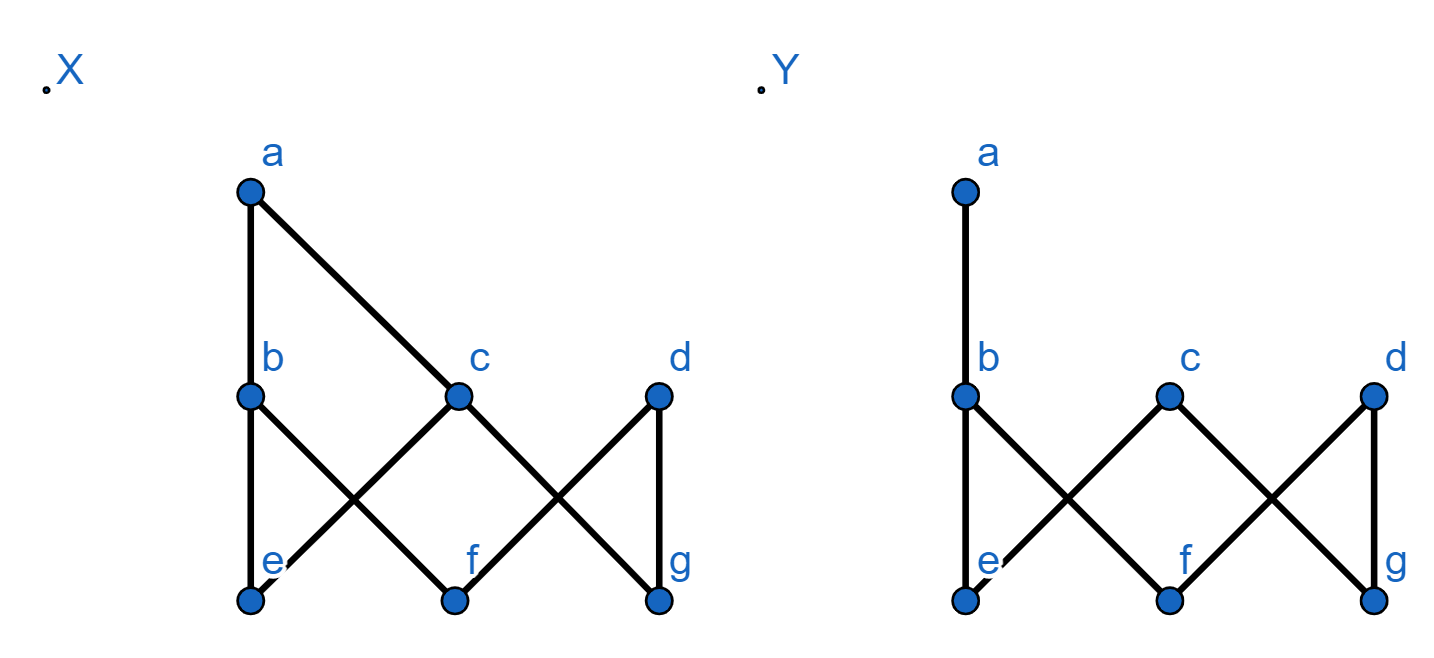
\includegraphics[width=0.6\linewidth]{xy.png}
    \end{figure}

Naslednjo zaporedje diagraov, nam pokaže, kako pridemo do jedra prostora $X$, z odstranjevanjem odvečnih točk. Točka $b$ je navzgor odvečna v $X$, $c$ je navzgor odvečna v $X\backslash\{b\}$, $e$ je pa navzgor odvečna v $X\backslash\{b,c\}$. Prostor $X\backslash \{b,c,e\}$ je minimalen končen prostor in je jedro od $X$.

\begin{figure}[h]
    \centering
    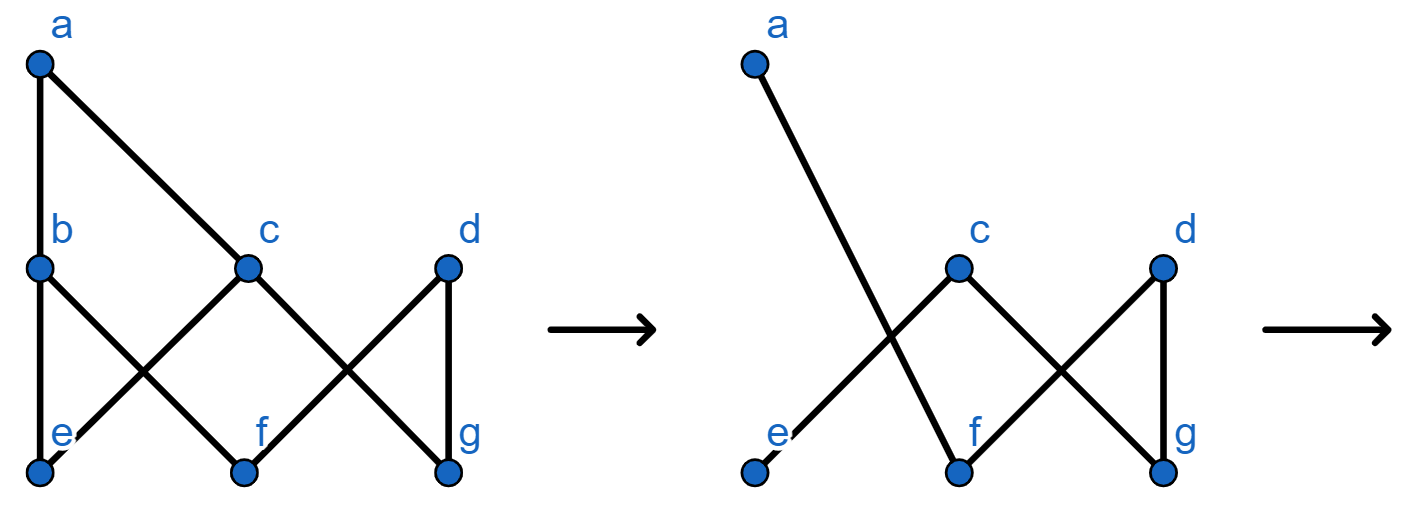
\includegraphics[width=0.6\linewidth]{prv.png}
    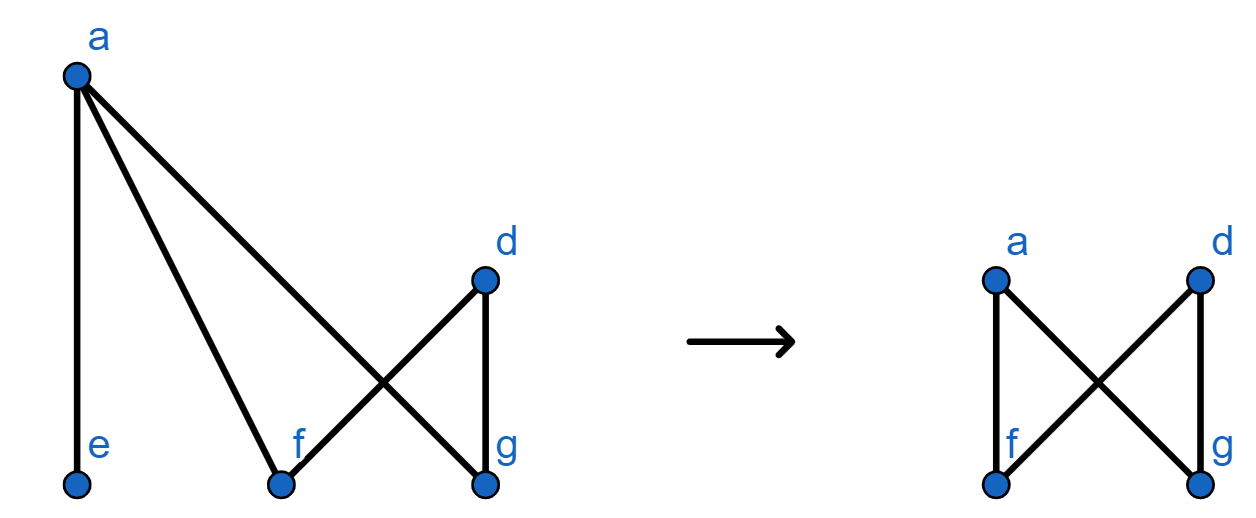
\includegraphics[width=0.6\linewidth]{drug.png}
\end{figure}

Po drugi strani pa je $a$ navzdol odvečna v $Y$ in $Y\backslash \{a\}$ je minimalen. $X$ in $Y$ nista homotopsko ekvivalentna, saj njuni jedri nista homeomorfni.
\end{primer}

%\begin{trditev}
%Naj bo $X$ končen $T_0$ prostor, potem je $X$ minimalen končen prostor, natanko tedaj, ko če $\forall x,y\in X$ velja, da če je  $\forall z\in X$ ki je primerljiv z $x$, primerljiv tudi z $y$, potem sledi da $x=y$
%\end{trditev}

%\begin{dokaz}
   
   % Najprej negiramo obe strani ekvivalence. predpostavimo, da $X$ ni minimalen, potem obstaja odvečna točka $x$. Brez škode za splošnost predpostavimo, da je $x$ navzdol odvečna in naj bo $y$ maksimum od $\hat{U}_x$. Če $z\geq x$, potem je $z\geq y$, če pa je $z\le x$, potem je $z\leq y$, ampak $x\neq y$.
%Recimo zdaj, da obstajata $x\neq y$, taka da je vsak element ki je primerljiv z $x$ primerljiv tudi z $y$, torej je tudi $x$ primerljiv z $y$. Predpostavimo $x>y$. Naj bo $A=\{z\in X |  z>x \text{ in za vsak $w\in X$, primerljiv z $z$, $z$ je primerljiv z $y$}\}$. $A$ je neprazna, saj je $x\in A$. Naj bo $x'$ minimalni element v $A$. Pokažimo, da je $x'$ navzdol odvečna točka in $y=\text{max}(\hat{U}_x)$. Naj bo zdaj $z<x'$, potem je $z$ primerljiv $y$, saj $x'\in A$. Recimo, da $z>y$ in naj bo $w\in X$. Če $w\geq z$, potem je $w\geq y$, torej $z\in A$, kar je pa v protislovju z minimalnostjo $x'$. Zato $z\leq y$, torej je $y$ maksimum v $\hat{U}_x$.
%\end{dokaz}
\section{Minimalni modeli prostorov}\label{sec:minimal}

\begin{definicija}
    Končni topološki prostor je \textit{model} prostora $X$, če mu je šibko homotopsko ekvivalenten. Model je \textit{minimalen}, če ima izmed vseh modelov najmanjšo kardinalnost.
\end{definicija}


\begin{definicija}
    Naj bo $X$ končen $T_0$ prostor. \textit{Simplicialni kompleks} $\mathcal{K}(X)$ \textit{prirejen X}, je simplicialni kompleks, čigar simpleksi so neprazne verige v $X$. Če je $f: X\rightarrow Y$ zvezna preslikava med dvema $T_0$ prostoroma. \textit{prirejena simplicialna preslikava} $\mathcal{K}(f):\mathcal{K}(X) \rightarrow \mathcal{K}(Y)$ definiramo kot $\mathcal{K}(f)(x) = f(x)$.
\end{definicija}
Vidimo, če je $f: X\rightarrow Y$ zvezna, je $\mathcal{K}(f):\mathcal{K}(X) \rightarrow \mathcal{K}(Y)$ simplicialna, saj ohranja ureditev in slika verige v verige.
Točka $\alpha$ v geometrijski realizaciji $|\K(X)|$ je
konveksna kombinacija oblike
$\alpha = t_1x_1+t_2x_2 + \ldots + t_r x_r$, pri čemer 
$\sum_{i=1}^{r}t_i=1$, $t_i \ge 0$ in 
velja, da je $x_1 < x_2 < \ldots < x_r$ veriga v $X$.
Nosilec $\alpha$ je množica supp($\alpha$)$= \{x_1,x_2,\ldots,x_r\}$. Pomembno vlogo igra 
 preslikava $\alpha \mapsto x_1$.
 
 \begin{definicija}
    Naj bo $X$ končen $T_0$ prostor, Definirajmo
    $\mathcal{K}$-\textit{McCordovo} preslikavo $\mu_X:|\mathcal{K}
    (X)|\rightarrow X$, z $\mu_X(\alpha) =$
    \text{min}(\text{supp}($\alpha))$.
\end{definicija}



\begin{izrek}{\textbf{McCordov}}\label{iz:mccord}
    Naj bosta $X$ in $Y$ topološka prostora in naj bo $f:X\rightarrow Y$ zvezna. Če je zožitev
    $$
    f|_{f^{-1}(U)}:f^{-1}(U)\rightarrow U
    $$
    šibka homotopska ekvivalenca za vsako bazno množico $U$, potem je $f:X\rightarrow Y$  šibka homotopska ekvivalenca.
\end{izrek}

\begin{opomba}
    Izrek ne velja le za zožitev na bazne množice, ampak tudi na vsako \textit{bazi podobno pokritje}, torej za vsako pokritje, ki je baza za kako drugo topologijo.
\end{opomba}



\begin{lema}\label{lem:sibka}
    Naj bo $x\in X$ in naj bo $L=X\ \backslash \
    U_x\subseteq \mathcal{K}(X)$. Potem se vsak $\alpha \in |\k(X)|\ \backslash \ |L|$ da napisati, kot $\alpha = t\beta + (1-t)\gamma$, za $\beta \in |\k(U_x)|, \ \gamma \in |L|$ in $0<t\leq 1$, pri čemer je $\alpha$ zvezno odvisna od $\beta, \gamma$ ter $t$ in $\beta, \gamma$ ter $t$ so enolično določeni.
\end{lema}
\begin{dokaz}
    $L$ je subkompleks, ki ga napenjajo oglišča, ki niso v $U_x$. Za vsak $\alpha \in |\k(X)|\ \backslash \ |L|$, 
    $$\alpha = \sum_{i=1}^{n} \alpha_i v_i 
    = \sum_{i=1}^{r} \alpha_i u_i + \sum_{i=r+1}^{n}\alpha_i v_i,\ \text{za}\ \sum_{i=1}^{n} \alpha_i=1,
    $$
    za $u_i \in U_x$, $v_i \in X \ \backslash \ U_x$ in za nek $r\in \{1,2, \cdots, n-1\}$. S t označimo $\sum_{i=1}^{r} \alpha_i$, torej je $1-t=\sum_{i=r+1}^{n} \alpha_i$ in $0<t\leq 1$. Potem $\beta =\sum_{i=1}^{r} \alpha_i u_i/t \in |\k(U_x)|$, saj je $\sum_{i=1}^{r} \alpha_i/t=1$ in podobno $\gamma=\sum_{i=r+1}^{n} 
    \alpha_i v_i/(1-t) \in |\k(X \ \backslash \ U_x)|$. Zveznost in enoličnost sledi iz konstrukcije.

\end{dokaz}

\begin{izrek}
    \label{iz:ksibka}
    $\mathcal{K}$-\textit{McCordova} preslikava je šibka homotopska 
    ekvivalenca za vsak končen $T_0$-prostor.
\end{izrek}

\begin{dokaz}
    Definirajmo retrakcijo $r:U_x\rightarrow \{x\}$ kot 
    $r(y)=x$, za vsak $y\in X$. Ker je $x$ maksimum v 
    $U_x$, je $r\geq 1_X$, zato je po trditvi 
    \ref{iz:ograje} $r\simeq 1_X$, torej je $U_x$ 
    kontraktibilna množica. Dokazali bomo, da je za vsak 
    $x\in X$, $\mu_X^{-1}(U_x)$ odprta in kontraktibilna. S 
    tem bomo pokazali, da je $\mu_X$ zvezna in da so 
    zožitve $\mu_X|_{\mu_X^{-1}(U_x)}:\mu_X^{-1}(U_x)\rightarrow 
    U_x$ šibke homotopske ekvivalence, kar pa po McCordovem izreku \ref*{iz:mccord}
    pomeni, da je preslikava $\mu_X$ šibka homotopska ekvivalenca.

    Naj bo $x\in X$ in naj bo $L=X\ \backslash \
    U_x\subseteq \mathcal{K}(X)$. $L$ je torej 
    subkompleks, ki ga napenjajo oglišča, ki niso v $U_x$. 
    Trdimo, da 
    $$
    \mu_X^{-1}(U_x)=|\mathcal{K}(X)|\ \backslash \ |L|.
    $$
    Pokažimo najprej, da $\mu_X^{-1}(U_x)\subseteq 
    |\mathcal{K}(X)|\ \backslash \ |L|$. Naj bo $\alpha \in 
    \mu_X^{-1}(U_x)$, torej je min$(\text{supp}
    (\alpha))\in U_x$, zato \text{supp}($\alpha$) vsebuje 
    oglišče iz $U_x$, zato $\alpha \notin |L|$, torej $\alpha 
    \in |\mathcal{K}(X)|\ \backslash \ |L|$.

    Pokažimo še, da $|\mathcal{K}(X)|\ \backslash \
    |L|\subseteq \mu_X^{-1}(U_x)$. Naj $\alpha \in |\mathcal{K}(X)|\ \backslash \ |L|.$
    Če  $\alpha \notin |L|$, potem obstaja $y\in 
    \text{supp}(\alpha)$, tak, da $y \in U_x$, zato je 
    min$(\text{supp}(\alpha))\leq y \leq x$, zato je 
    $\mu_X(\alpha) \in U_x$ in $\alpha \in \mu_X^{-1}
    (U_x)$.
    Ker je $|L|$ zaprta podmnožica $|\mathcal{K}(X)|$, je 
    $\mu_X^{-1}(U_x)$ odprta.

    Pokažimo, da je $\mu_X^{-1}(U_x)$ kontrabilna. Prvo pokažimo, da je 
    $|\mathcal{K}(U_x)|$ krepki deformacijski retrakt 
    od $|\mathcal{K}(X)|\ \backslash \ |L|$. Naj bo $i:|\k(U_x)|\hookrightarrow |\mathcal{K}
    (X)|\ \backslash \ |L|$ inkluzija. Če je $\alpha \in |\mathcal{K}(X)|\ 
    \backslash \ |L|$, potem je po lemi \ref{lem:sibka}  $\alpha = t\beta + 
    (1-t)\gamma$, za $\beta \in |\k(U_x)|, \ \gamma \in |L|$ in $0<t\leq 1$. 
    Definirajmo $r:|\mathcal{K}(X)|\ \backslash \ |L|\rightarrow |\k(U_x)|$ 
    kot $r(\alpha)=\beta$. Ker je $\alpha$ zvezna in je zožitev $r|_{(|\mathcal{K}(X)|\ \backslash \ |L|)\cap 
    \overline{\sigma}}:(|\mathcal{K}(X)|\ \backslash \ |L|)\cap 
    \overline{\sigma} \rightarrow \overline{\sigma}$ zvezna, za vsak 
    $\sigma \in \k(X)$, sledi da je $r$ zvezna. Definirajmo zdaj linearno homotopijo $H:(|\mathcal{K}(X)|\ \backslash \ |L|) \times I \rightarrow (|\mathcal{K}(X)|\ \backslash \ |L|)$ med $1_{(|\mathcal{K}(X)|\ \backslash \ |L|)}$ in $ir$ kot 
    $$
    H(\alpha,s)=(1-s)\alpha + s\beta.
    $$
    H je dobro definirana, in zvezna, saj je vsaka zožitev 
    $$
    H|_{((|\mathcal{K}(X)|\ \backslash \ |L|)\cap 
    \overline{\sigma})\times I}:((|\mathcal{K}(X)|\ \backslash \ |L|)\cap 
    \overline{\sigma})\times I \rightarrow \overline{\sigma}
    $$
    dobro definirana in zvezna, $\sigma \in \k(X)$.

    Ker je vsak element iz $U_x$ primerljiv z $x$, je $\k(U_x)$ 
    simplicialni stožec, zato je po trditvi \ref{pos:kontr} $|\k(U_x)|$ 
    kontraktibilen in zato je kontraktibilna tudi $\mu_X^{-1}
    (U_x)=|\mathcal{K}(X)|\ \backslash \ |L|$.
\end{dokaz}


Če imamo končen topološki prostor $X$, mu priredimo simplicialni kompleks
$\k(X)$, Geometrijska realizacija $|\k(X)|$ tega kompleksa pa je šibko homotopsko ekvivalentna 
začetnemu prostoru $X$. Torej lahko za vsak prostor, ki je homeomorfen geometrijski realizaciji
nekega simplicialnega kompleksa, najdemo njegov končen model tj. končen topološki prostor, ki mu
je šibko homotopsko ekvivalenten.

\begin{figure}[h]
    \centering
    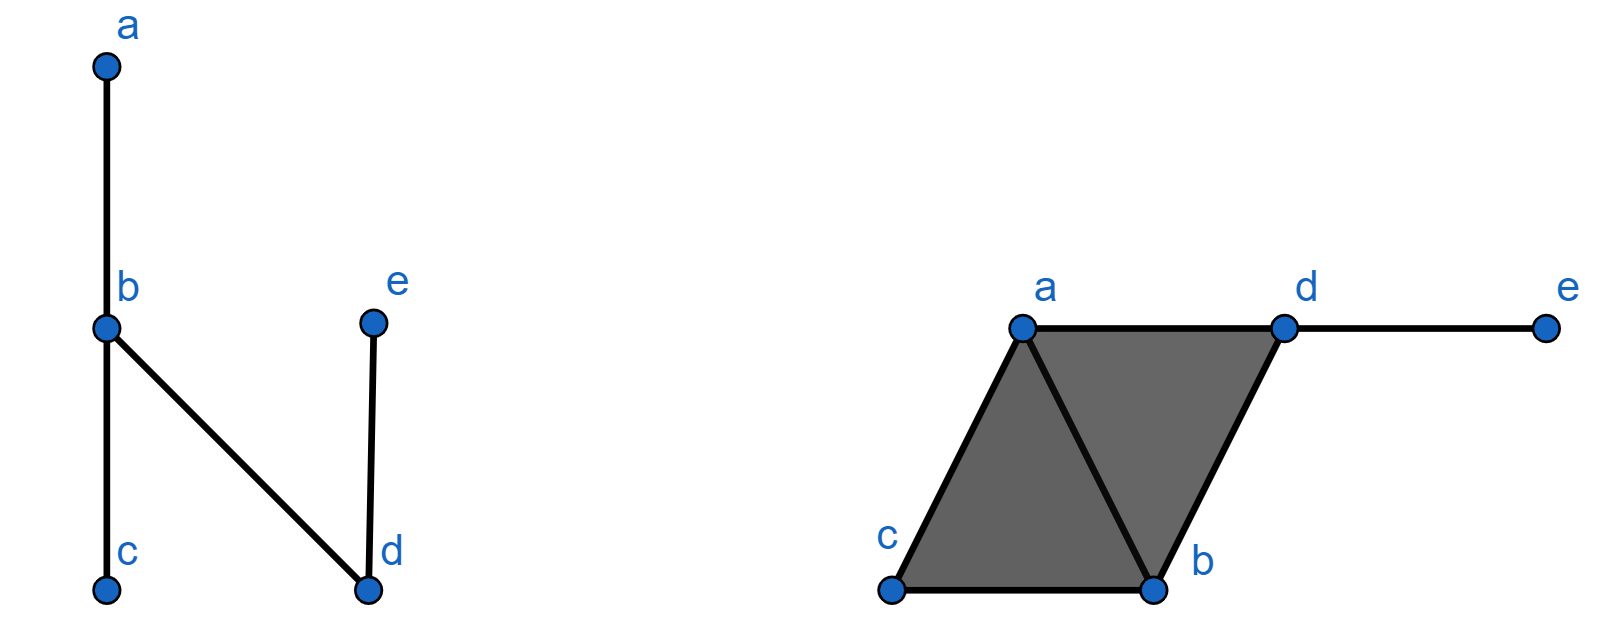
\includegraphics[width=1\linewidth]{simp.png}
    \caption{Končen prostor in njegov prirejen simplicialni kompleks, ki mu je šibko homotopsko ekvivalenten.}
\end{figure}


\begin{definicija}
    Naj bo $K$ končen simplicialni kompleks. Končen $T_0$
    prostor $\chi(K)$ prirejen $K$, je delno urejena množica simpleksov v $K$, urejena glede na inkluzijo.
    Naj bo $\varphi:K\rightarrow L$ simplicialna preslikava, potem preslikavo  $\chi(\varphi):\chi(K)\rightarrow \chi(L)$ definiramo kot 
    $\chi(\varphi)(\sigma)=\varphi(\sigma)$ za vsak simpleks $\sigma \in K$
\end{definicija}


\begin{lema}
    \label{lem:komutira}
    Naj bo $f :X\rightarrow Y$ zvezna preslikava med dvema $T_0$ prostoroma, potem naslednji diagram komutira

    \[\begin{tikzcd}
        {|\k(X)|}\arrow{r}{|\k(f)|} \arrow[swap]{d}{\mu_X} & {|\k(Y)|} \arrow{d}{\mu_Y} \\
       X \arrow{r}{f} & Y
       \end{tikzcd}
       \]
    
\end{lema}



\begin{dokaz}
    \begin{align*}
        f\mu_X(\alpha)&=f(\text{min}(\text{supp}(\alpha)))\overset{*}{=}\text{min}(f(\text{supp}(\alpha))) \\
        &=\text{min}(\text{supp}(|\k(f)|(\alpha)))=\mu_Y|\k(f)|(\alpha)
    \end{align*}

    Pri čemer $*$ velja zaradi zveznosti $f$, druge enakosti pa veljajo kar po definiciji.
\end{dokaz}

Če je $K$ končen kompleks, potem je $\k(\chi(K))$ prva baricentrična subdivizija.
definirajmo $\chi$-\textit{McCordovo preslikavo} $\mu_K=\mu_{\chi(K)}S_K^{-1}: |K|\rightarrow \chi(K)$. 
Ker je kompozitum dveh šibkih homotopskih ekvivalenc tudi šibka homotopska ekvivalenca, takoj sledi naslednji izrek.

\begin{izrek}
    \label{iz:xsibka}
    $\chi$-McCordova preslkava $\mu_K$ je šibka homotopska
     ekvivalenca za vsak končen simplicialni kompleks $K$.
\end{izrek}


\begin{trditev}
    Naj bo $\varphi: K\rightarrow L$ simplicialna preslikava med končnima kompleksoma. Potem naslednji diagram komutira do homotopije natančno
    \\
  
\[\begin{tikzcd}
    {|K|} \arrow{r}{|\varphi|} \arrow[swap]{d}{\mu_K} & {|L|} \arrow{d}{\mu_L} \\
    \chi(K) \arrow{r}{\chi(\varphi)} & \chi(L)
    \end{tikzcd}
    \]
\end{trditev}

\begin{proof}
    Najprej poiščimo homotopijo med $|\varphi|s_K$ in $s_L|\varphi'|$, kjer je $\varphi'=\k(\chi(\varphi))$ preslikava med baricentričnima subdivizijama $K'$ in $L'$.
    Naj bo $S=\{\sigma_1,\sigma_2,\cdots,\sigma_r\}$ simpleks 
    v $K'$ in naj bo $\sigma_1 \subsetneq \sigma_2 \subsetneq 
    \cdots \subsetneq \sigma_r$ veriga simpleksov iz $K$. Naj bo $\alpha$
    točka v zaprtem simpleksu $\overline{S}$. Potem je $S_K(\alpha)
    \in \overline{\sigma_r}\subseteq |K|$ in  $|\varphi|S_K(\alpha) \in 
    \overline{\varphi(\sigma_r)}\subseteq |L|.$ \
    Velja pa tudi $|\varphi'|(\alpha)\in \{\varphi(\sigma_1)$$,\varphi(\sigma_2),\cdots,\varphi(\sigma_r)\}$
    in potem $S_L|\varphi'|(\alpha) \in \overline{\varphi(\sigma_r)}.$ Zato 
    je linearna homotopija



    \begin{centering}
        $$
        H:|K'|\times I \rightarrow |L| \\
        H: (\alpha,t) \mapsto (1-t)|\varphi|S_K(\alpha) + tS_L|\varphi'|(\alpha)\\
        $$
    \end{centering}
zvezna in dobro definirana in zato $|\varphi|S_K(\alpha) \simeq 
S_L|\varphi'|$. Iz leme \ref{lem:komutira} sledi, da naslednji diagram komutira 
\[\begin{tikzcd}[row sep=large, column sep=large]
    {|\k(\chi(K))|}\arrow{r}
   {|\k(\chi(\varphi)|} \arrow[swap]{d}{\mu_{\chi(K)}} & {|\k(\chi(L))|} \arrow{d}{\mu_{\chi(L)}} \\
   \chi(K) \arrow{r}{\chi(\varphi)} & \chi(L)
   \end{tikzcd}
   \]
in zato

\begin{align*}
    \mu_L|\varphi|=\mu_{\chi(L)}S_L^{-1}|\varphi| \simeq \mu_{\chi(L)}|\varphi'&|S_K^{-1} \\
    =\chi(\varphi)\mu_{\chi(K)}S_K^{-1} =\chi(\varphi)\mu_K&
  \end{align*}
\end{proof}

Iz lastnosti 2 od 3 in dejstva, da je preslikava, ki je homotopna šibki homotopski ekvivalenci isto šibka homotopska ekvivalenca, takoj sledi naslednja trditev.

\begin{trditev}
    Naj bo $\varphi : K\rightarrow L$ simplicialna preslikava med končnima kompleksoma, potem je $|\varphi|$ šibka homotopska ekvivalenca, natanko tedaj, ko je $\chi(\varphi)$ šibka homotopska ekvivalenca.
\end{trditev}

Iz izrekov \ref{iz:xsibka} in \ref{iz:ksibka} pa takoj sledi naslednji posledici.

\begin{posledica}
    \begin{itemize}

        \item Naj bosta $X$ in $Y$ končna $T_0$ prostora. Potem sta $X$ in $Y$ šibko homotopsko ekvivalentna, natanko tedaj, ko sta $|\k(X)|$ in $|\k(Y)|$ homotopsko ekvivalentna.
        \item Naj bosta $K$ in $L$ končna simplicialna kompleksa. Potem sta $|K|$ in $|L|$ homotopsko ekvivalentna, natanko tedaj, ko sta $\chi(K)$ in $\chi(L)$ šibko homotopsko ekvivalentna
    \end{itemize}
\end{posledica}

\section{Konstrukcije novih topoloških prostorov}


V tem poglavju bomo definirali nekaj osnovnih konstrukcij iz algebraične topologije in jih uporabili na simplicialnih kompleksih ter končnih in splošnih topoloških prostorih. S $S^n$ označimo $n-$dimenzionalno sfero.

\textit{Spoj} Topoloških prostorov $X$ in $Y$ je topološki prostor $X\ast Y = X\times Y 
\times I /_{\sim}$, pri čemer $(x, y_1, 0) \sim (x, y_2, 0)$ in  $(x_1, y, 1) \sim (x2, y, 1)$. 
Torej $X\times Y\times \{0\}$ strnemo na $X$ in $X\times Y\times \{1\}$ na $Y$. Intuitivno, 
to pomeni, da vsako točko na $X$ z intervalom povežemo z vsako točko na $Y$.
Poseben primer spoja je \textit{suspenzija} $\Sigma X$, ki je spoj $X$ in prostora na dveh točkah, $S^0$.

$$
\Sigma X=S^0\ast X = X\times I /_{(X\times \{0\},X\times \{1\})}
$$

\begin{figure}[h]
    \centering
    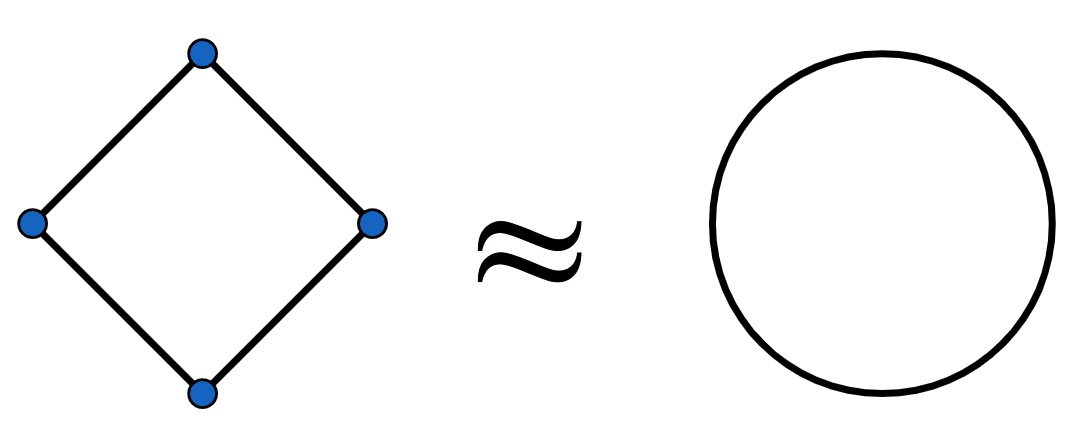
\includegraphics[width=0.6\linewidth]{homeo2.png}
    \caption{Suspenzija $\Sigma S^0$ je homeomorfna $S^1$. V splošnem velja $\Sigma S^n=S^{n+1}$}
\end{figure}

Naj bosta $X$ in $Y$ topološka prostora in $x_0\in X$ ter $y_0\in Y$, potem je 
\textit{Šop} $X\bigvee Y$ kvocient disjunktne unije $X\bigsqcup Y$, pri
 katerem identificiramo $x_0$ in $y_0$. Na primer $S^1\bigvee S^1$ je prostor,
  ki ga dobimo, če staknemo dve krožnici v eni točki in je homeomorfen "\textbf{8}".


\textit{Simplicialni spoj $K\ast L$} kompleksov $K$ in $L$ z disjunktnima množicama oglišč je kompleks.

$$
K\ast L=K\cup L \cup \{\sigma \cup \tau| \sigma \in K, \tau \in L \}
$$

\textit{Simplicialni stožec} $aK$ z bazo $K$ je spoj $K$ in oglišča $a\notin K$


\begin{trditev}
    \label{tr:spoj}
    Naj bosta $K$ in $L$ končna simplicialna kompleksa, potem je geometrijska realizacija $|K\ast L|$ homeomorfna topološkemu spoju $|K|\ast |L|$.
\end{trditev}
\begin{dokaz}
Definirajmo $f:|K|\times |L|\times I\rightarrow |K\ast L|$, kot $f(k,l,j)=jk+(1-j)l$. Če $k=\Sigma_{i=1}^n \alpha_i v_i$ in $l=\Sigma_{i=1}^m \beta_i u_i$, potem je $\{v_i|\text{ $\alpha_i > 0$}\}$ simpleks v $K$ in $\{u_i|\text{ $\beta_i > 0$}\}$ simpleks v $L$ ter $\Sigma_{i=1}^n \alpha_i = \Sigma_{i=1}^m \beta_i=1$. Zato je $\{v_i|\text{ $\alpha_i > 0$}\}\cup \{u_i|\text{ $\beta_i > 0$}\}$ simpleks v $K\ast L$  in $\Sigma_{i=1}^n \alpha_i j + \Sigma_{i=1}^m \beta_i (1-j)=1$. Torej je $f$ dobro definirana. Velja tudi $f(k,l,0)=l$, neodvisno od $k$ in $f(k',l',1)=k'$, neodvisno od $l'$, torej $f$ slika ekvivalenčne razrede v točke. Ker sta $K$ in $L$ končna kompleksa, je $|K|\times |L|\times I$ kompaktna, torej $f$ slika iz kompakta v $T_2$ prostor in je zato zaprta. Preslikava $f$ je zaprta in surjektivna, zato je kvocientna. Naredi iste identifikacije kot $q$, zato je inducirana preslikava$\overline{f}$ dobro definirana in je homeomorfizem.

\[\begin{tikzcd}
    {|K|\times |L|\times I }\arrow{r}{f} \arrow[swap]{d}{q} & {|K\ast L|} \\
    {|K|\ast |L|} \arrow{ru}{\overline{f}}
   \end{tikzcd}
   \]


\end{dokaz}

Če je $K$ 0-kompleks z dvema ogliščema, potem je $|K\ast L|=|K|\ast |L|=S^0\ast |L| = \Sigma |L|$.

\begin{figure}[h]
    \centering
    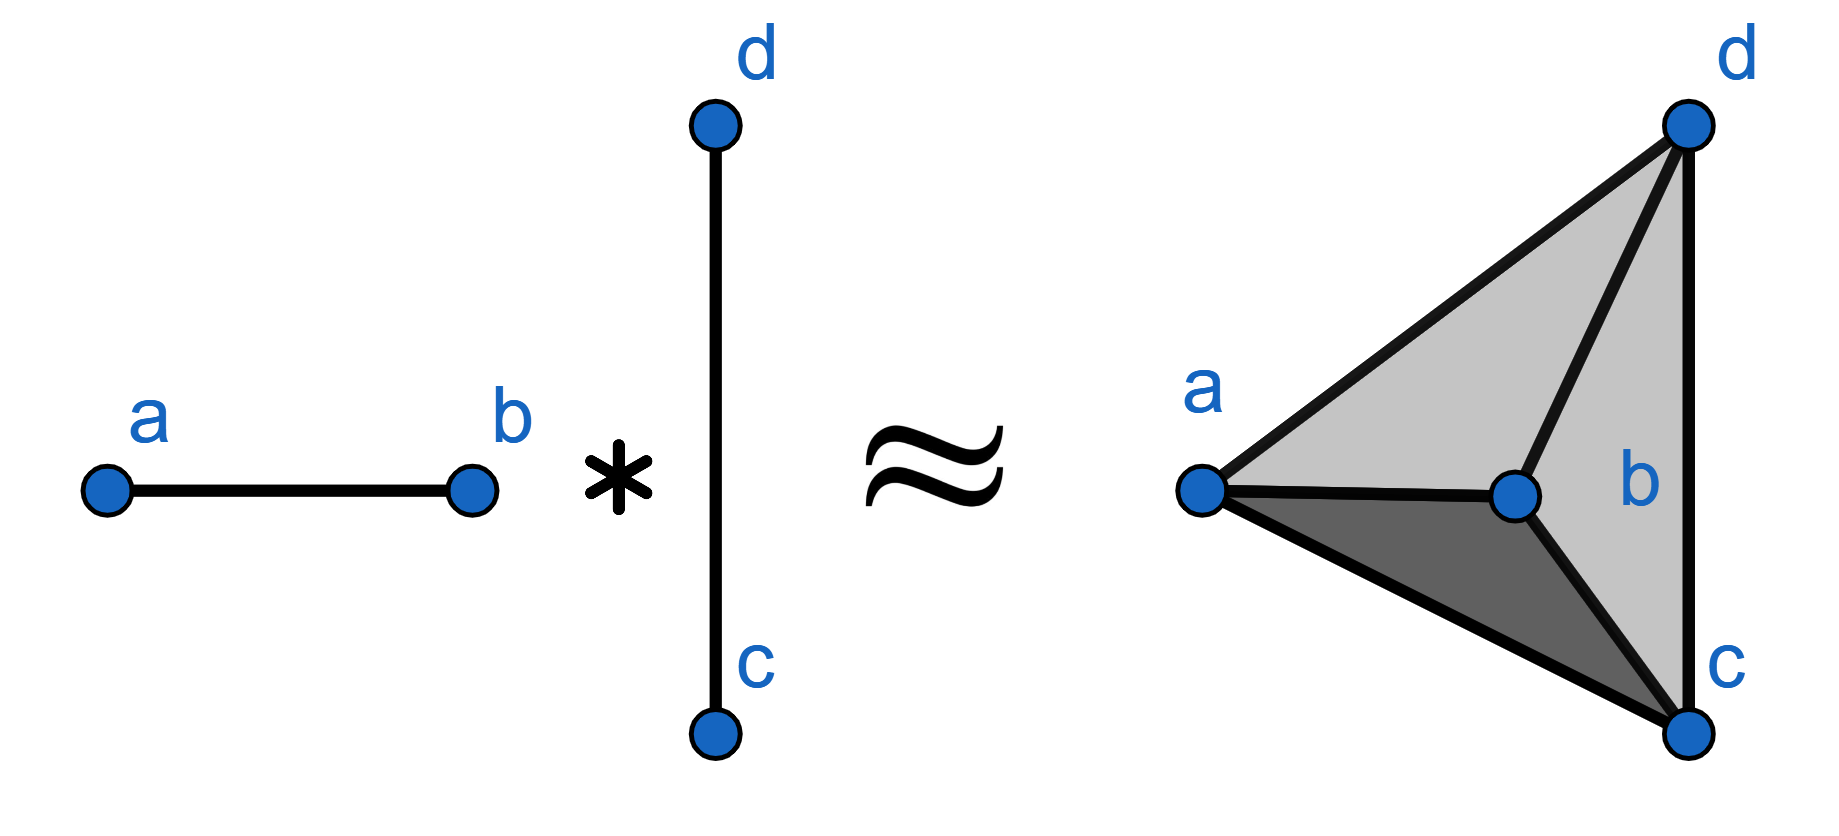
\includegraphics[width=0.6\linewidth]{spoj.png}
    \caption{Spoj dveh $1-$simpleksov je $3-$simpleks.}
\end{figure}

\begin{definicija}
    \textit{Ne-Hausdorffov spoj} $X\circledast Y$ dveh končnih $T_0-$prostorov
     $X$ in $Y$ je disjunktna unija $X\bigsqcup Y$, v kateri
     pustimo ureditev v $X$ in v $Y$ in nastavimo $x\leq y$ za vsaka 
     $x\in X$ in $y\in Y$.
\end{definicija}
Ta spoj je asociativen in v splošnem ni komutativen, tako kot pri topološkem
 in simplicialnem spoju imamo poseben primer ne-Hausdorffovega ne-Hausdorffove Suspenzije
  $\mathds{S}(X)=X \circledast S^0$.

  Ne-Hausdorffova suspenzija reda $n$ je definirana rekurzivno, kot  $\mathds{S}^n=\mathds{S}(\mathds{S}^{n-1}(X))$.
  \begin{opomba}
    \label{op:spoj}
    Velja $\k(X\circledast Y) = \k(Y)\ast \k(X)$.
  \end{opomba}
\section{Minimalni model sfere}


\begin{definicija}
    Končni topološki prostor je \textit{model} prostora $X$, če mu je šibko homotopsko ekvivalenten. Model je \textit{minimalen}, če ima izmed vseh modelov najmanjšo kardinalnost.
\end{definicija}

Spomnimo se, da je minimalni končni prostor, prostor brez odvečnih točk, ker pa je vsak končen prostor homotopsko ekvivalenten svojemu jedru, sledi, da je vsak minimalni končni model prostora tudi minimalen končen prostor.

\begin{trditev}
    Končen prostor $\mathds{S}^n(S^0)$ je končni model n-dimenzionalne sfere $S^n$ za vsak $n\geq 0$
\end{trditev}

\begin{dokaz}
    Vemo že, da je $\mathds{S}^n(S^0)$ šibko homotopsko ekvivalenten $|\k(\mathds{S}^n(S^0))|$,
    po opombi \ref{op:spoj} in trditvi \ref{tr:spoj} pa velja $|\k(\mathds{S}^n(S^0))|=|\k(\underbrace{S^0\circledast S^0 \circledast \cdots \circledast S^0}_\text{$n+1$-krat})|=
    |\k(S^0)\ast\k(S^0) \ast \cdots \ast \k(S^0)|=|\k(S^0)|\ast
    |\k(S^0)| \ast \cdots \ast |\k(S^0)|=S^0\ast
    S^0 \ast \cdots \ast S^0=S^n$
\end{dokaz}

Zdaj bomo še dokazali, da je $\mathds{S}^n(S^0)$ minimalni končni model za $S^n$. Še več, pokazali bomo, da ima vsak prostor, šibko homotopsko ekvivalenten $S^n$ vsaj $2n+2$ točk, če ima pa natanko $2n+2$ točk pa je homeomorfen $\mathds{S}^n(S^0)$.

\begin{definicija}
    \textit{Višina} $\htt(X)$ končne delno urejene množice je ena manj kot dožina najdaljše verige v $X$. Z $\# X$ pa označimo število elementov v $X$.
\end{definicija}
Dimenzija prirejenega kompleksa $\k(X)$ je enaka $\htt(X)$.


\begin{izrek}
    Naj bo $X\neq\ast$ minimalen prostor, potem ima vsaj $2\htt(X)+2$ točk. Če ima natanko $2\htt(X)+2$ točk, potem je homeomorfen $\mathds{S}^{\htt(X)}(S^0)$
\end{izrek}    

\begin{dokaz}
    Naj bo $x_0<x_1 <\cdots <x_h$ veriga dolžine $h=\htt(X)$. Ker je $X$
     minimalen, $x_i$ ni odvečna točka za noben $0\leq i <h$. Potem za 
     vsak $0\leq i <h$ obstaja $y_{i+1}$, tak da $y_{i+1}> x_i$ $(1)$ in $y_{i+1}
     \ngeq x_{i+1}$. Trdimo, da so vse točke $y_i$ med seboj različne, za vsak
      $0< i \leq h$ in da nobena ni enaka $x_j$ za noben $0\leq j \leq h$.

      Ker $y_{i+1} > x_i$, sledi, da $y_{i+1}\neq x_j$ za noben $j\leq i$, 
      ker velja tudi $y_{i+1}\ngeq x_{i+1}$ pa sledi, da $y_{i+1}\neq x_j$ za 
      noben $j> i$

      Če je $y_{i+1}= y_{j+1}$ za nek $i<j$, potem je $y_{i+1}= y_{j+1}\geq
       x_j \geq x_{i+1}$, kar je pa v protislovju z $y_{i+1} 
       \ngeq x_{i+1}$.

       Ker je vsak končen prostor z minimumom ali z maksimumom kontraktibilen 
       in je $X\neq \ast$, minimalen prostor, sledi da $X$ nima minimuma, 
       torej mora obstajati točka $y_0\in X$, za katero velja $y_0 \ngeq x_0$.
        Zato je $y_0$ različna od drugih $2h+1$ točk in zato $\# X\geq 2h+2$.
        Predpodstavimo zdaj, da ima $X$ natanko $2h+2$ točk, torej 
        $$
        X=\{x_0,x_1,\cdots x_h,y_0,y_1,\cdots y_h,\}
        $$
        Če bi bil $x_i < y_i$, za $0<i\leq h$ bi bilo to v nasprotju z 
        maksimalnostjo verige $x_0 <\cdots <x_h$, saj bi potem veljalo $x_{i-1} 
        < y_i < x_i$. Tudi $y_i \ngtr x_i$ za $0\leq i \leq h$ zaradi (1), zato sta $x_i $ in $y_i$ neprimerljiva za $0\leq i \leq h$.

        Z indukcijo na $j$ pokažimo, da $y_i < x_j$ in $y_i < y_j$za vse $i<j$. Za $j=0$ 
        ni kaj za dokazovati. Naj bo $0\leq k <h$ in recimo, da trditev drži za $j=k$, 
        dokažimo, da drži tudi za $j=k+1$. Ker $x_{k+1}$ ni navzdol odvečna, 
        obstaja $z$, da $z< x_{k+1}$ in $z\nleq x_k$, ker sta $x_{k+1}$ in 
        $y_{k+1}$ neprimerljiva, velja tudi $z\neq y_{k+1}$. Iz indukcijske 
        predpodstavke sledi, da je vsaka točka, z izjemo $y_k$ in $y_{k+1}$, večja 
        od $x_{k+1}$ ali manjša od $x_k$. Ker $y_{k+1} \nleq x_{k+1}$, je potem
        $z=y_k$ in zato $y_k<x_{k+1}$. Dokažimo še, da $y_k\leq y_{k+1}$. Ker 
        $y_{k+1}$ ni navzdol odvečna, obstaja $w\in X$, da je $w<y_{k+1}$ in 
        $w\nleq x_k$. Iz indukcijske predpodstavke
         in dejstva, da $y_{k+1}\ngeq x_{k+1}$, sklepamo,
        da $w=y_k$ in zato $y_k<y_{k+1}$. Za $i<k$ pa velja $y_i<x_k<x_{k+1}$ in
        $y_i<x_k<y_{k+1}$.

        Dokazali smo, da za vsak $i<j$,  velja $y_i < x_j,\ y_i < y_j,\ x_i < x_j$ in
        $x_i < y_j$ ter da sta $x_i$ in $y_i$ neprimerljiva za vsak $0\leq j \leq h$.
        To je pa ureditev v $\mathds{S}^h(S^0)$ in zato je $X$ homeomorfen 
        $\mathds{S}^h(S^0)$.

\end{dokaz}

\begin{figure}[h]
    \centering
    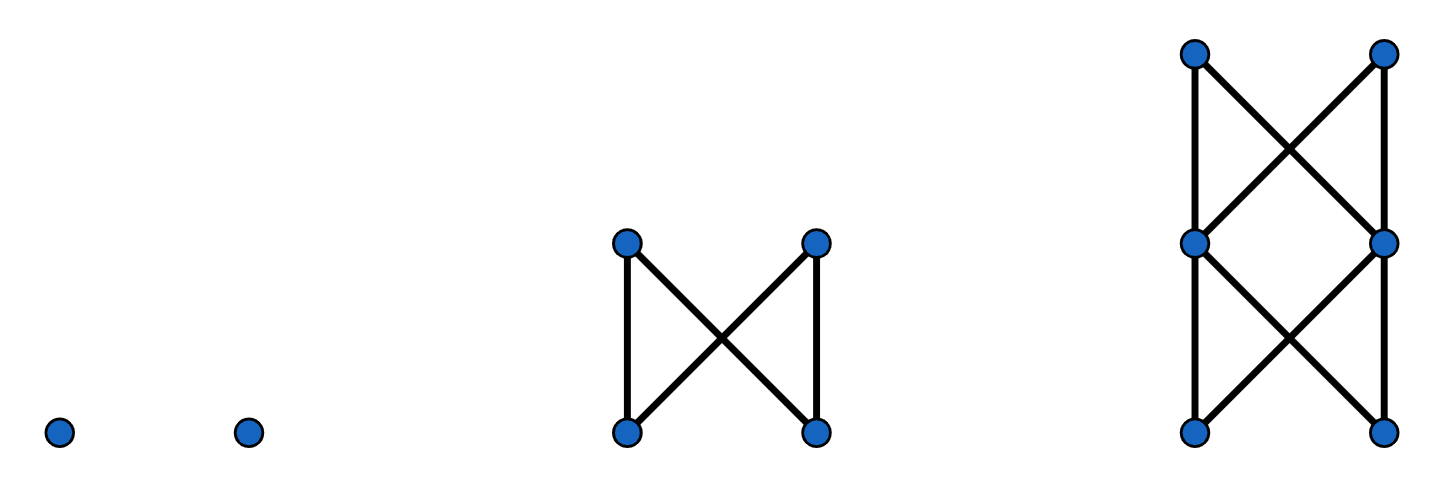
\includegraphics[width=0.8\linewidth]{sfere.png}
    \caption{Minimalni modeli za $S^0$, $S^1$ in $S^2$.}
\end{figure}

Ker je $\mathds{S}^n(S^0)$ model za $S^n$, čigar višina je enaka $n$ in ima 
$2n+2$ točk, je $\mathds{S}^n(S^0)$ minimalni model za $S^n$. Model je 
enoličen, saj je vsak model za $S^n$ na $2n+2$ točkah homeomorfen 
$\mathds{S}^n(S^0)$.
\section{Zanke v Hassejevem diagramu}\label{sec:hasse}

Pokazali bomo, kako se fundamentalna grupa končnega $T_0$ 
prostora izraža preko prirejenega Hassejevega diagrama.
Hassejev diagram končnega $T_0$ prostora $X$ označimo z 
$\h(X)$, z $E(\h(X))$ pa označimo množico njegovih robov.


\begin{definicija}
    Naj bo $(X,x_0)$ končen pointed $T_0$ prostor. Urejen par 
$e=(x,y)$ imenujemo $\mathcal{H}-$rob od $X$, če $(x,y)\in 
E(\mathcal{H}(\mathcal{X}))$, ali $(y,x)\in 
E(\h(X))$. Točki $x$ rečemo \textit{začetek} $x$ in označimo 
$x=\mathfrak{o}(e)$, točki $y$ pa \textit{konec} od $e$, 
označimo $\mathfrak{e}(e)=y$. \textit{Inverz} $\h-$roba $e=(x,y)$ je $\h-$rob $e^{-1}=(y,x)$

$\h-$pot v $(X,x_0)$ je zaporedje (lahko tudi prazno), $\h-$robov $\xi=e_1e_2\cdots e_n$, 
za katerega velja, da je $\mathfrak{e}(e_i)=\mathfrak{o}(e_{i+1})$, za vsak $0\leq i \leq n-1$.
 Začetek $\h-$poti $\xi$ je  $\mathfrak{o}(\xi)=e_1$, konec pa $\mathfrak{e}(\xi)=e_n$, 
 začetek in konec prazne poti je $\mathfrak{o}(\emptyset)=\mathfrak{e}(\emptyset)=x_0$
 Če je $\xi=e_1,e_2\cdots e_n$ $\h-$pot, definiramo $\overline{\xi}=e_n^{-1},\cdots 
 e_2^{-1}e_n^{-1}$. Če sta $\xi$ in $\xi'$ $\h-$poti in velja $\mathfrak{e}(\xi)=
 \mathfrak{e}(\xi')$, lahko definiramo produktno \pot $\xi\xi'$, kot zaporednje 
 $\h-$robov v $\xi$, ki mu sledi zaporednje $\h-$robov v $\xi'$.

 Za \pot $\xi=e_1e_2,\cdots e_n$ pravimo, da je \textit{monotona}, če je $e_i\in 
 E(\h(X))$ za vsak $1\leq i \leq n$ ali pa je $e_i^{-1}\in E(\h(X))$ za vsak $1\leq i \leq n$.
 \textit{Zanka} iz $x_0$ je \pot, ki se začne in konča v $x_0$. Za zanki $\xi$ in
  $\xi'$ rečemo, da sta blizu, če obstajajo monotone $\h-$poti $\xi_1,\xi_2,\xi_3,\xi_4$,
   take, da  sta množici $\{\xi,\xi'\}$ in $\{\xi_1\xi_2\xi_3\xi_4,\xi_1\xi_4\}$ enaki.

   Rečemo, da sta zanki $\xi$ in $\xi'$ $\h-$ekvivalentni, če obstaja končno zaporednje zank $\xi=\xi_1,\xi_2,...,\xi_n=\xi'$, tako da sta vsaki zaporedni zanki blizu. Z $\langle\xi\rangle$ označimo $\h-$ ekvivalenčni razred zanke $\xi$ in z $\mathscr{H}(X,x_0)$ množico teh razredov.
\end{definicija}

    \begin{figure}[h!]
          \centering
          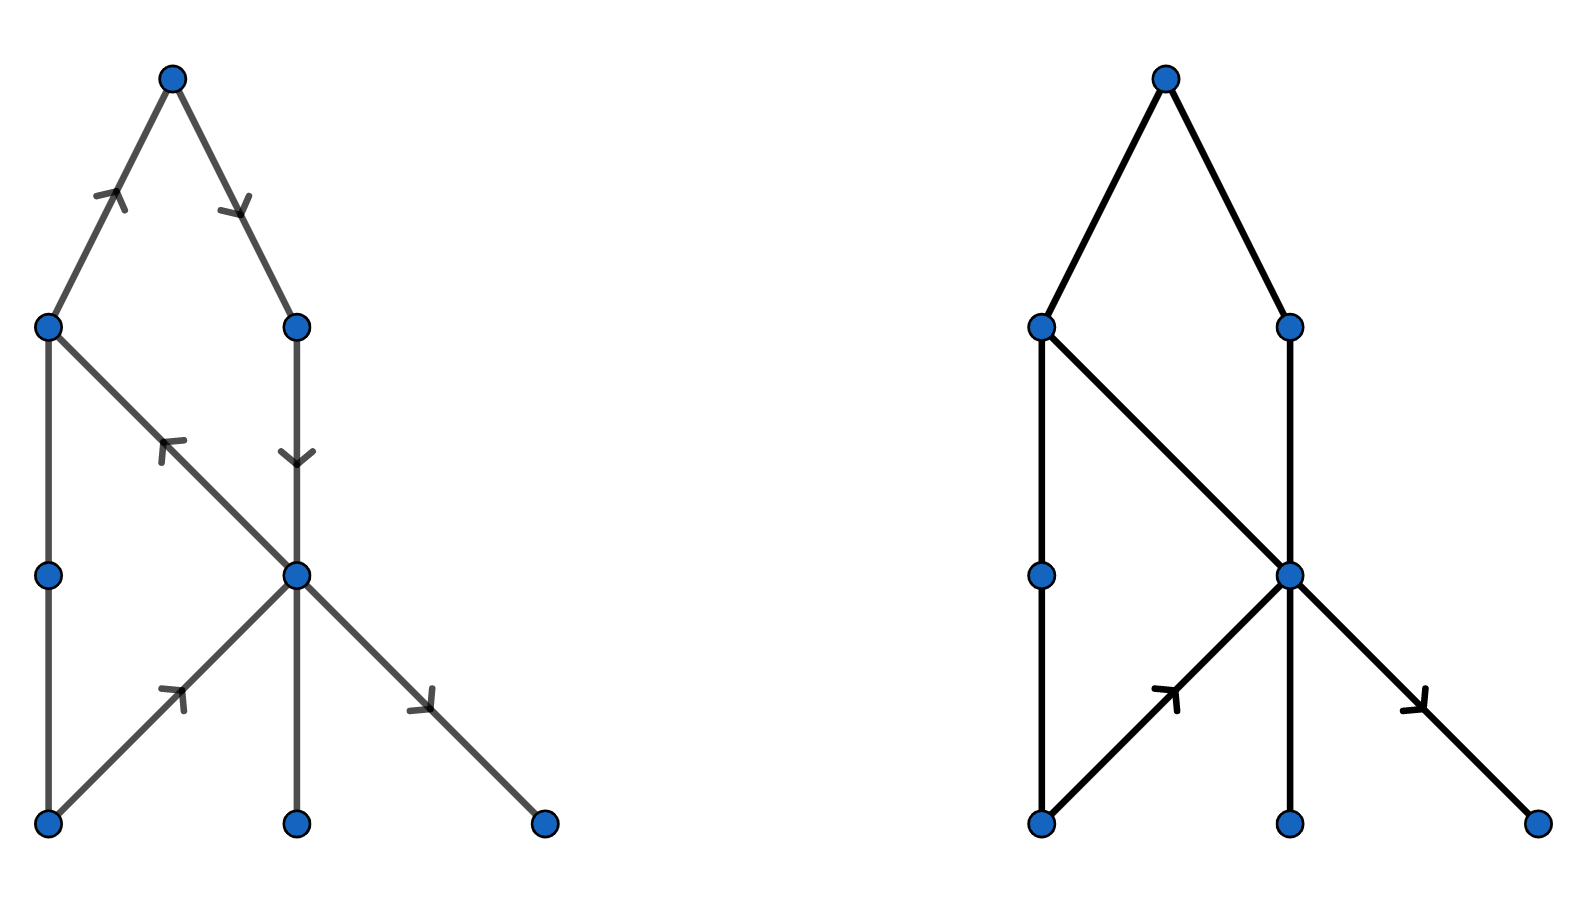
\includegraphics[width=0.6\linewidth]{poti.png}
        \caption{Primer poti ki sta blizu}
        \end{figure}

\begin{izrek}
    Naj bo $(X,x_0)$ končen pointed $T_0$ prostor. Potem je množenje $\langle\xi\rangle\langle\xi'\rangle=\langle\xi\xi'\rangle$ dobro definirano in inducira grupno strukturo na $\mathscr{H}(X,x_0)$
\end{izrek}

\begin{dokaz}
    Dobra definiranost in asociativnost sta očitni, enota je $\langle\emptyset\rangle$. Naj bosta $\xi$ in $\xi'$ poti, $e$ $\h-$rob in $\mathfrak{e}(\xi)=\mathfrak{o}(\xi')=\mathfrak{o}(e)$. potem sta poti $\langle\xi \xi'\rangle$ in $\langle\xi e e^{-1} \xi'\rangle$ blizu, saj je $e$ monotona pot. Iz tega takoj sledi, da je inverz od $\langle e_1 e_2...e_n\rangle$ enak $\langle e_n^{-1}...e_2^{-1}e_1^{-1}\rangle$.
\end{dokaz}


\begin{izrek}
    Naj bo $(X,x_0)$ končen pointed $T_0$ prostor. Potem je grupa sklenjenih lomljenk $E(\k(X),x_0)$ izomorfna $\mathscr{H}(X,x_0)$.
\end{izrek}

\begin{dokaz}
    Definirajmo 
    \begin{align*}
\varphi:\mathscr{H}(X,x_0)&\rightarrow E(\k(X),x_0)\\
\langle e_1e_2...e_n\rangle&\mapsto [e_1e_2...e_n]\\
\emptyset &\mapsto [(x_0,x_0)]
    \end{align*}.

    Najprej pokažimo, da je $\varphi$ dobro definiran.
    Naj bosta zanki $\xi_1 \xi_2 \xi_3 \xi_4$ in $\xi_1 \xi_4 $ blizu in naj bosta $\xi_2 = e_1e_2...e_n$ in $\xi_3 = e'_1e'_2...e'_m$ monotoni $\h-$poti. Potem velja 
\begin{align*}
    [\xi_1 \xi_2 \xi_3 \xi_4]&=[\xi_1 e_1e_2...e_{n-1}(\mathfrak{o}(e_n)\mathfrak{e}(e_n)) \xi_3 \xi_4]\\
    &=[\xi_1 e_1e_2...e_{n-2}(\mathfrak{o}(e_{n-1})\mathfrak{e}(e_n)) \xi_3 \xi_4]=\cdots=[\xi_1(\mathfrak{e}(\xi_1)\mathfrak{e}(e_n)) \xi_3 \xi_4],
\end{align*}
saj je $\{\mathfrak{o}(e_{n-1}),\mathfrak{o}(e_{n-1+1}),\mathfrak{e}(e_{n-i+1})\}$, analogno 
$$
[\xi_1(\mathfrak{e}(\xi_1)\mathfrak{e}(e_n)) \xi_3 \xi_4]=[\xi_1(\mathfrak{e}(\xi_1)\mathfrak{e}(e_n))( \mathfrak{o}(e'_1)\mathfrak{o}(\xi_4)) \xi_4]
$$
in zato 
\begin{align*}
    [\xi_1 \xi_2 \xi_3 \xi_4]&=[\xi_1(\mathfrak{e}(\xi_1)\mathfrak{e}(e_n)) (\mathfrak{o}(e'_n)\mathfrak{o}(\xi_4)) \xi_4]\\
    &=[\xi_1(\mathfrak{e}(\xi_1)\mathfrak{e}(e_n)) (\mathfrak{e}(e_n)\mathfrak{e}(\xi_1)) \xi_4]=[\xi_1(\mathfrak{e}(\xi_1) \mathfrak{e}(\xi_1)) \xi_4]=[\xi_1 \xi_4].
\end{align*}


Obratno, če je $\xi =(x_0,x_1)(x_1,x_2)...(x_{n-1},x_n)$ lomljenka v $\k(X)$ z $x_0=x_n$, potem sta $x_i$ in $x_{i-1}$ primerljiva za vsak $1\leq i \leq n$, zato lahko najdemo monotone $\h-$poti $\xi_1, \xi_2,... \xi_n$, take da $\mathfrak{o}(x_{i-1})=\mathfrak{e}(x_i)$ za $1\leq i \leq n$. Definirajmo

\begin{align*}
    \psi: E(\k(X),x_0)&\rightarrow \mathscr{H}(X,x_0),\\
    [\xi]&\mapsto \langle\xi_1, \xi_2,... \xi_n\rangle.
\end{align*}

Definicija je neodvisna od izbire $\h-$poti $\xi_i$, saj če se izbiri razlikujeta za kak $i=k$, potem sta $\xi_1...\xi_k...\xi_n$ in $\xi_1...\xi'_k...\xi_n$ $\h-$ekvivalentni, saj sta obe blizu $\xi_1...\xi_k\xi_k^{-1}\xi_k...\xi_n$, torej $\langle \xi_1...\xi_k...\xi_n \rangle = \langle \xi_1...\xi'_k...\xi_n \rangle$

Definicija je neodvisna od izbire predstavnika. Recimo da sta $\xi(x,y)(y,z)\xi'$ in $\xi(x,z)\xi'$ ekvivalentni lomljenki v $\k(X)$, ki se začneta in končata v $x_0$, pri čemer sta $\xi$ in $\xi'$ lomljenki, $x,y$ in $z$ pa so primerljivi.
Če $y$ leži med $x$ in $z$, lahko najdemo monotono $\mathcal{H}-$pot od $x$ do $z$, ki vsebuje $y$ in nadomesti \pot od $x$ do $y$ in od $y$ do $z$ in zato je $\psi$ ekvivalentno definirana na $\xi(x,y)(y,x)\xi'$ in $\xi(x,z)\xi'$.
Če je $z\leq x \leq y$ lahko poiščemo monotone $\mathcal{H}-$poti $\alpha$ od $x$ do $y$ in $\beta$ od $z$ do $x$, potem bo $\overline{\alpha}\overline{\beta}$ nadomestila pot $(y,z)$ in $\overline{\beta}$ bo nadomestila pot $(x,z)$. Dokazati moramo le še, da velja $\langle\gamma \alpha \overline{\alpha}\overline{\beta}\gamma'\rangle=\langle \gamma\overline{\beta}\gamma\rangle$, za $\h-$poti $\gamma$ in $\gamma'$, kar je pa trivialno. Preostale kombinacije $x,y$ in $z$ dokažemo analogno.

Očitno sta $\varphi$ in $\psi$ drug drugemu inverzna in zato sta izomorfizma.
\end{dokaz}

Ker sta grupi $E(\k(X),x_0)$ in $\pi_1(|\k(X)|,x_0)$ izomorfni, takoj sledi naslednji rezultat.

\begin{posledica}
    Naj bo $(X,x_0)$ končen pointed $T_0$ prostor, potem $\pi_1(X,x_0)=\mathscr{H}(X,x_0)$.
\end{posledica}
\section{Minimalni modeli grafov}

Graf v topologiji je topološki prostor, ki ga dobimo iz običajnega grafa 
$G=(E,V)$, če oglišča iz $V$ zamenjamo s točkami in vsako povezavo $e\in 
E$, $e=xy$, za $x,y\in V$, zamenjamo z enotskim intervalom, pri čemer 
identificiramo $0$ in $x$ ter $1$ in $y$.
Graf je torej geometrijska realizacija enodimenzionalnega simplicialnega 
kompleksa. Graf je končen, če ima končno mnogo oglišč. 

Brez dokaza bomo upoštevali dejstvo, da je za enodimenzionalne poliedre 
šibki homotopski tip odvisen le od fundamente grupe, kar pomeni, da sta 
sta prostora šibko homotopsko ekvivalentna, natanko tedaj, ko imata 
izomorfni fundamentalni grupi.


\begin{definicija}
    Naj bo $K$ simplicialni kompleks dimenzije $n$ in naj $s_m$ označuje število $m-$simpleksov v $K$.
    \textit{Eulerjeva karakteristika} $\chi(K)$ simplicialnega kompleksa $K$, je  $\chi(X)=\sum\limits_{i=0}^n (-1)^m s_m$
\end{definicija}

Če se omejimo na enodimenzionalne simplicialne komplekse oziroma grafe, 
potem je eulerjeva karakteristika enaka $V-E$, kjer je $V$ število 
oglišč, $E$ pa 
število robov v grafu. Eulerjeva karakteristika dreves je enaka 1.

\begin{trditev}
    Naj bo $G$ topološki graf in $e$ njegova povezava. Potem je
    $G\times \{0\}\cup e\times I$ deformacijski retrakt od $G\times I$.
\end{trditev}

\begin{dokaz}
    Obstaja retrakcija $r: I\times I \rightarrow I\times \{0\} \cup \partial I \times I$, na primer radialna projekcija iz točke $(1/2,2)\in I\times \mathbb{R}$. Ta retrakcija nam porodi deformacijsko retrakcijo $r^1_t=tr+(1-t)1$, ta deformacijska retrakcija nam porodi deformacijsko retrakcijo $G\times I \rightarrow G\times\{0\} \cup {V\cup e \times I}$, kjer je $V$ množica ogliščč grafa. Ker je $\{v\}\times I$ kontraktibilna, obstaja deformacijska retrakcija $r^2_t: G\times\{0\} \cup {V\cup e \times I}\rightarrow G\times\{0\} \cup { e \times I}$. Če izvedemo $r_t^1$ v času $[0,1/2]$ in $r^2_t$ v $[1/2,1]$, dobimo deformacijsko retrakcijo $r_t:G\times I \rightarrow G\times\{0\} \cup {e \times I}$. Retrakcija je zvezna, saj je zvezna kot zožitev na vse robove in na vsa oglišča v $G$, oziroma na vse zaprte simplekse.
\end{dokaz}

\begin{trditev}
    Naj bo $G$ končen topološki graf in  $e=\{u,v\}$ povezava v grafu za $u\neq v$, potem se vsak par preslikav $G\times \{0\}\rightarrow G$ in $e\times I \rightarrow G$, ki sovpada na $e\times \{0\}$, da razširiti do preslikave $G\times I \rightarrow G$
\end{trditev}

\begin{dokaz}
    Ker je $e$ zaprt v $G$, lahko preslikavi združimo v preslikavo $G\times \{0\}\cup e\times I\rightarrow G$, ki je zvezna, saj je zvezna na zaprtih podprostorih $G\times \{0\}$ in $e\times I$. Če to komponiramo z retrakcijo $G\times I \rightarrow G\times \{0\}\cup e\times I$, dobimo razširitev $G\times I \rightarrow G.$
\end{dokaz}

Recimo, da imamo preslikavo $f_0:G\rightarrow G$ in homotopijo $f_t:e\rightarrow G$, preslikave $f_0|A$, potem nam ta trditev pove, da lahko to homotopijo razširimo do homotopije $f_t:G\rightarrow G$ dane preslikave $f_0$.

\begin{trditev}
    Naj bo $G$ končen topološki graf in  $e=\{u,v\}$ povezava v grafu za $u\neq v$. Potem sta prostora $G$ in $G/_e$ homotopsko ekvivalentna.
\end{trditev}

\begin{dokaz}
    Naj bo $i:e\rightarrow G$ inkluzija. Povezava $e$ je kontraktibilna, torej obstaja homotopija $r_t:e \rightarrow e$ in $r_0=1_e$. Naj bo $f_t:G\rightarrow G$ razširitev homotopije $ir_t$ in naj velja $f_0=1_G$.

    Ker $f_t(e)\subseteq e$, zato kompozicija $qf_t:G\rightarrow G/_e$ slika $e$ v točko, zato obstaja $\bar{f}_t:G/_e\rightarrow G/_e$, taka da velja $gf_t=\bar{f}_tq$. Pri $t=1$ je $f_1(e)$ enaka točki, v katero se $e$ kontrakira. Zato $f_1$ inducira preslikavo $g:G/_e \rightarrow G$, da velja $gq=f_1$.
    \begin{minipage}{0.4\textwidth}
        \centering
        $\begin{tikzcd}
            {G}\arrow{r}{f_t} \arrow[swap]{d}{q} & {G} \arrow{d}{q} \\
            G/_e \arrow{r}{\overline{f}_t} & G/_e
        \end{tikzcd}
        $
    \end{minipage}
    \begin{minipage}{0.4\textwidth}
        \centering
        $\begin{tikzcd}
            {G}\arrow{r}{f_1} \arrow[swap]{d}{q} & {G} \arrow{d}{q} \\
            G/_e \arrow{ru}{g} \arrow{r}{\overline{f}_1} & G/_e
        \end{tikzcd}
        $
    \end{minipage}
    
    Ker velja $qg(\bar{x})=qgq(x)=qf_1(x)=\bar{f}_1 q(x)=\bar{f}_1(\bar{x})$, sledi, da je $qg=\bar{f}_1$. Zato sta $q$ in $g$ homotopska inverza, saj je $gq=f_1\simeq f_0=1_G$ in $qg=\bar{f}_1\simeq \bar{f}_0 = 1_{G/_e}$
\end{dokaz}

\begin{posledica}
    Naj bo $G$ končen graf, in naj bo $T$ vpeto drevo. Potem sta 
    prostora $G$ in $G/_T$ homotopsko ekvivalentna.
\end{posledica}

Naj bo $T$ vpeto drevo grafa $G$. Velja $\chi(T)=1$. $G$ dobimo iz $T$ tako, da mu dodajamo povezave 
oziroma $1-$simplekse, zato $\chi(G)=1-n$, kjer je $n$ število povezav v $G$, ki niso v 
$T$. Prostor $G/_e$ dobimo iz $G$, tako da krajišči povezave zlepimo v eno točko, povezavo pa 
izbrišemo, torej ima nov prostor eno oglišče in eno povezavo manj, zato se eulerjeva karakteristika 
ohranja. $G/_T$ je prostor z enim ogliščem $x_0$ in $n$ povezavami, ki se začnejo in končajo v istem 
oglišču, torej je homeomorfen šopu $n=1-\chi(G)$ krožnic, kar označimo z $\bigvee\limits_{i=1}^{n}S^1$.

\begin{posledica}
    \label{pos:karakteristika}
    Šibki homotopski tip grafa je odvisen le od eulerjeve karakteristike
\end{posledica}

Minimalni model grafa je torej enak minimalnemu modelu  $\bigvee\limits_{i=1}^{n}S^1$. Poglejmo si 
fundamentalno grupo  $\pi_1(\bigvee\limits_{i=1}^{n}S^1,x_0)$, kjer je $x_0$ točka, v kateri so krožnice 
staknjene. Vsak ekvivalenčni razred zank predstavimo z zaporedjem krožnic, ki jih prepotuje in s 
smerjo v kateri gre čez krožnico. Če s $s_i$ označimo ekvivalenčni razred zanke čez $i-$to krožnico, potem lahko ekvivalenčni 
zank  predstavimo kot zaporedje $s_{i_1}^{j_1}s_{i_2}^{j_2}\cdots s_{i_m}^{j_m}$, za $m\in N$ in 
$j\in \{-1,1\}.$ Tu $j$ označuje smer po kateri gremo čez krožnico. Stik zank 
$s_{i_1}^{j_1}\cdots s_{i_m}^{j_m}$ in $s_{k_1}^{l_1}\cdots s_{k_m'}^{l_h}$ pa je ekvivalenten 
stiku zaporedij $s_{i_1}^{j_1}\cdots s_{i_m}^{j_m}s_{k_1}^{l_1}\cdots s_{k_m'}^{l_h}$.
Seveda velja $s_i s_i^{-1}=s_i^{-1}s_i=1$, kjer $1$ predstavlja trivialno zanko. 
Torej vidimo, da je fundamentalna grupa $\pi_1(\bigvee\limits_{i=1}^{n}S^1,x_0)$ enaka prosti grupi z $n$
generatorji, ki jo označimo z $F_n$.

\begin{trditev}
    Naj bo $X$ povezan topološki prostor in naj $x,x_0\in X, x\neq x_0$, taka da $x$ ni niti maksimalen, niti minimalen. Potem inkluzija asociiranih simplicialnih kompleksov $\k(X\backslash\{x\})\subseteq \k(X)$ inducira epimorfizem 
    $$
i_\star:E(\k(X\backslash\{x\}),x_0)\rightarrow E(\k(X),x_0)
    $$
    med njunima grupama sklenjenih lomljenk.
\end{trditev}

\begin{dokaz}
    Pokazati moramo, da je vsaka lomljenka v $\k(X)$ z izhodiščem $x_0$ ekvivalentna neki drugi lomljenki, ki ne gre skozi $x$.
    Recimo, da je $y\leq x$ in je $(y,x)(x,z)$ lomljenka v $\k(X)$. Če je $x\leq z$, potem je $(y,z)(x,z)\equiv(y,z)$, saj je $\{x,y,z\}$ simpleks. Če je pa $z< x$, potem obstaja $w>x$, saj $x$ ni maksimalen. Zato je $(y,x)(x,z)\equiv(y,x)(x,w)(w,x)(x,z)\equiv (y,w)(w,z)$. Če je $y\geq x$ je dokaz analogen.
\end{dokaz}

Če povezanemu prostoru $X$ postopoma odstranjujemo točke, ki niso minimalne ali maksimalne, v vsakem koraku dobimo epimorfizem med fundamentalnima grupama, ki pa ni nujno izomorfizem, saj imamo lahko v $\k(X\backslash\{x\})$ dve neekvivalentni zanki, ki sta v $\k(X)$ ekvivalentni.



\begin{posledica}
    Naj bo $X$ povezan končen $T_0$ prostor. Potem obstaja povezan $T_0$ prostor $Y\subseteq X$, višine kvečjemu $1$ in epimorfizem iz $\pi_1(Y,x)$ v $\pi_1(X,x)$.
\end{posledica}

\begin{trditev}
    Naj bo $n\in\mathbb{N}$. Če je $X$ minimalen model za 
    $\bigvee\limits_{i=1}^{n}S^1$, potem $\htt(X)=1$.
\end{trditev}

\begin{dokaz}
    Naj bo $X$ minimalen model za $\bigvee\limits_{i=1}^{n}S^1$. Potem obstaja povezan $T_0$ podprostor $Y\subseteq X$ višine $1$ in epimorfizem iz $\pi_1(Y,x)$ v $\pi_1(X,x)=F_n$.
Ker je $\htt(Y)=1$, je $Y$ model grafa, torej $\pi_1(Y,x)=F_m$, za $m\geq n$.

    V $\h(Y)$ imamo $m$ robov, ki niso v vpetem drevesu prirejenega grafa $\k(Y)$, zato lahko odstranimo $m-n$ robov iz $\h(Y)$ tako, da ostane povezan in dobljen prostor $Z$ je model za $\bigvee\limits_{i=1}^{n}S^1$.

    Velja $\#Z=\#Y\leq \#X$, ampak ker je $X$ končen minimalen model, mora veljati $\#X\leq\#Z$ in zato $X=Z$, torej je višina $X$ enaka 1.
\end{dokaz}
Z $\# X$ bomo označevali število elementov v množici $X$.

Naj bo $X$ minimalen model za $\bigvee\limits_{i=1}^{n}S^1$. Vpeljimo naslednje oznake, $i:=\#\{y\in X| y \text{ je minimalen}\}$ in $j:=\#\{y\in X| y \text{ je maksimalen}\}$. Potem $\#X=i+j$ in $\#E(\h(X))\leq ij$. Ker je $\chi(X)=1-n$, velja $n\leq 1 - (i+j) + ij=(i-1)(j-1)$. Navedimo glavni izrek razdelka.

\begin{izrek}
    Naj bo $n\in\mathbb{N}$. Končen $T_0-$prostor $X$ je minimalni model za  $\bigvee\limits_{i=1}^{n}S^1$ natanko tedaj, ko je $\htt(X)=1$, $\#X\geq\min\{i+j|(i-1)(j-1)\geq n\}$ in $\#E(\h(X))= \#X + n -1.$
\end{izrek}

\begin{dokaz}
    Pokazali smo že, da če je $X$ minimalen model za $\bigvee\limits_{i=1}^{n}S^1$, potem $\htt(X)=1$ in $\#X=\min\{i+j|(i-1)(j-1)\geq n\}$. 
    Če sta $i$ in $j$ taka, da $(i-1)(j-1)\geq n$, potem definiramo prostor $Y=\{x_1,x_2,...x_i,y_1,y_2,...y_j\}$ z ureditvijo $y_k<x_l$ 
    za vse $k$ in $l$, ki je model za $\bigvee\limits_{i=1}^{(i-1)(j-1)}S^1$. Potem lahko odstranimo $(i-1)(j-1)-n$ robov iz $\h(X)$ in tako dobimo povezan prostor kardinalnosti $i+j$, ki je model za $\bigvee\limits_{i=1}^{n}S^1$. Torej $\#X\leq \#Y=i+j$. To drži za vsaka $i$ in $j$, za katera velja $n\leq (i-1)(j-1)$, zato $\#X=\min\{i+j|(i-1)(j-1)\geq n\}$, zaradi minimalnosti $X$. $\#E(\h(X))= \#X + n -1$ pa sledi, ker $\chi(X)= 1-n$.

    Dokažimo še v drugo smer. Naj velja  $\htt(X)=1$, $\#X=\min\{i+j|(i-1)(j-1)\geq n\}$ in $\#E(\h(X))= \#X + n -1.$ Dokazati moramo le, da je $X$ povezan, saj potem iz prve in tretje predpodstavke sledi, da je $X$ model za  $\bigvee\limits_{i=1}^{n}S^1$, iz druge pa sledi, da je model minimalen.

    Naj bodo $X_l$ komponente povezanosti od $X$, za $1\leq l \leq k$. Z $M_l$ označimo množico maksimalnih elementov v $X_l$, z $m_l$ pa $X\backslash M_l$. Naj $i= \sum\limits_{l=1}^k \# M_l$ in $j= \sum\limits_{l=1}^k \# m_l$. Ker $i+j=\# X =\min \{s+t|(s-1)(t-1)\geq n\}$, sledi, da $(i-2)(j-1)<n=\# E(\h(X))-\# X +1=\#E(\h(X)) -(i+j) +1$ in zato $ij -\# E(\h(X))<j-1$. To pomeni, da se $\k(X)$ od polnega dvodelnega grafa $(\cup m_l,\cup M_l)$
    razlikuje v manj kot $j-1$ robovih. Ker za $r\neq l$ ne obstaja povezava med ogliščem v $m_l$ in ogliščem v $M_r$, velja
    $$
        j-1>\sum\limits_{l=1}^{k}\# M(j- \# m_l)\geq \sum\limits_{l=1}^{k}(j- \# m_l)=(k-1)j.
    $$

    Zato $k=1$ in dokaz je končan.
\end{dokaz}
\begin{primer}
    \begin{figure}[h]
        \centering
        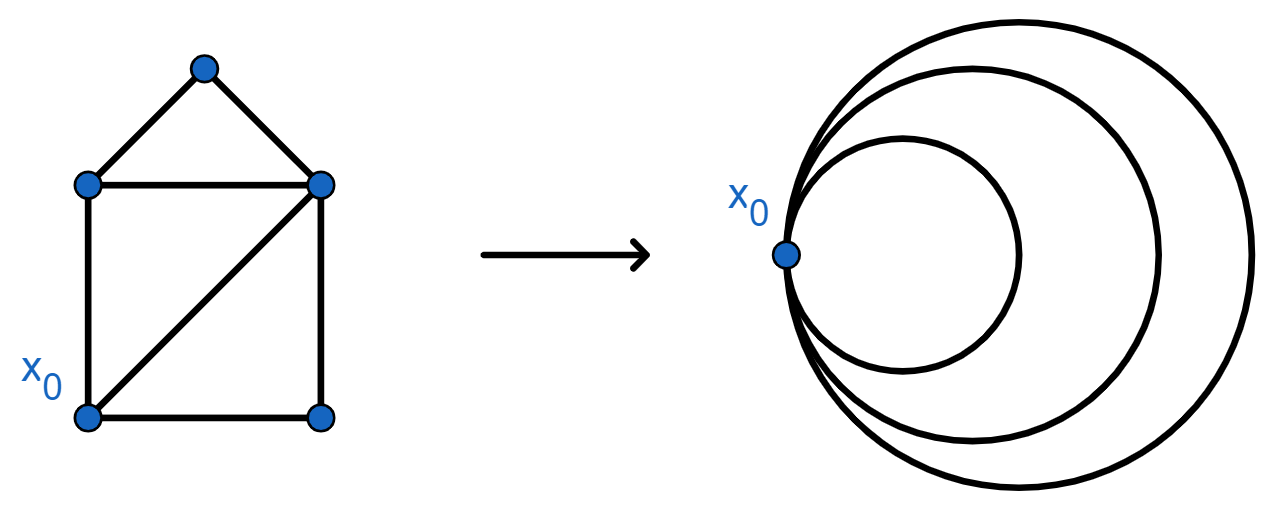
\includegraphics[width=0.55\linewidth]{v3.png}
    \end{figure}
    \begin{figure}[h]
        \centering
        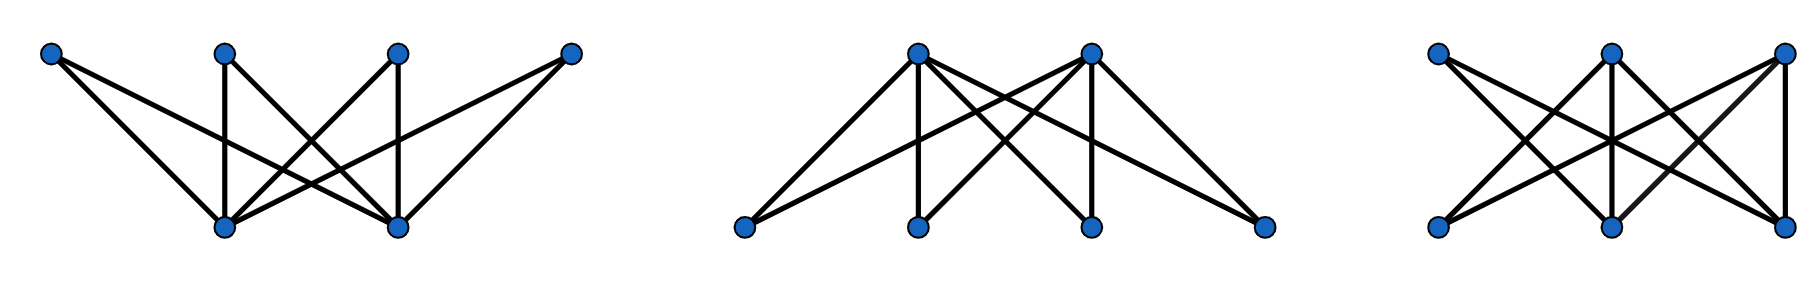
\includegraphics[width=0.8\linewidth]{grafi.png}
    \end{figure}

    Graf na sliki ima eulerjevo karakteristiko enako $-2$, zato je homotopsko ekvivalenten spoju $3$ krožnic, $\bigvee\limits_{i=1}^{3}S^1$. Vsak model za $\bigvee\limits_{i=1}^{3}S^1$ ima $6$ točk in $8$ robov, ker obstajajo trije nehomeomorfni končni prostori s temi lastnosti vidimo, da graf v splošnem nima enolično določenega minimalnega modela.
\end{primer}
\geslo{edge path}{lomljenka}
\geslo{edge path group}{grupa sklenjenih lomljenk}
\geslo{down set}{navzdol zaprta množica}
\geslo{Euler characteristic}{Eulerjeva karakteristika}
\geslo{homotopy equivalence}{homotopska ekvivalenca}
\geslo{join}{spoj}
\geslo{simplicial complex}{simplicialni kompleks}
\geslo{up set}{navzgor zaprta množica}
\geslo{weak homotopy equivalence}{šibka homotopska ekvivalenca}
\geslo{wedge sum}{šop}
\geslo{$\h-$path}{\pot}


\nocite{*}
\bibliography{refs}
%\bibliographystyle{plain}

\tableofcontents
\section*{Slovar strokovnih izrazov}





\end{document}